\documentclass[11pt]{article}

\usepackage[T1]{fontenc}
\usepackage[margin=1in]{geometry}
\usepackage{amsmath,amssymb,mathtools,amsthm}
\usepackage{booktabs,tabularx,array}
% microtype font expansion requires a scalable T1 font; fall back if lmodern is absent.
\IfFileExists{lmodern.sty}
  {\usepackage{lmodern}\usepackage{microtype}}
  {\usepackage[expansion=false]{microtype}}
\usepackage{enumitem}
\usepackage{tikz}
\usepackage{pgfplots}
\pgfplotsset{compat=1.16}
\usepackage[hidelinks]{hyperref}

\setlength{\parindent}{0pt}
\setlength{\parskip}{0.65em}
\setlist[itemize]{leftmargin=*,itemsep=0.2em,topsep=0.3em}
\setlist[enumerate]{leftmargin=*,itemsep=0.3em,topsep=0.3em}
\renewcommand{\arraystretch}{1.18}
\setcounter{tocdepth}{1}

\newcommand{\AP}{\operatorname{AP}}
\newcommand{\CAP}{\operatorname{CAP}}
\newcommand{\Regime}{\mathcal{R}}
\newcommand{\Tpi}{\CAP_{\pi_\star}}
\newcommand{\E}{\mathbb{E}}
\newcommand{\iid}{\mathrel{\overset{\mathrm{iid}}{\sim}}}

% Full notation, used at the point of definition.
\newcommand{\RCAPfull}{\operatorname{R\text{-}CAP}^{\mathrm{sup}}_{\Regime,\pi_\star}}
% Reduced notation, used in running text once the regime is fixed.
\newcommand{\RCAP}{\operatorname{R\text{-}CAP}^{\mathrm{sup}}_{\pi_\star}}
\newcommand{\RCAPHat}{\widehat{\operatorname{R\text{-}CAP}}{}^{\,\mathrm{sup}}_{\pi_\star}}
\newcommand{\RCAPHatB}{\widehat{\operatorname{R\text{-}CAP}}{}^{\,\mathrm{sup}}_{\pi_\star,B}}
\newcommand{\RCAPnull}{\operatorname{R\text{-}CAP}^{\mathrm{sup,null}}_{\pi_\star}}
\newcommand{\RCAPnullHat}{\widehat{\operatorname{R\text{-}CAP}}{}^{\,\mathrm{sup,null}}_{\pi_\star}}
\newcommand{\RCAPcalHat}{\widehat{\operatorname{R\text{-}CAP}}_{\pi_\star}}

\newcommand{\PRep}{P_{\mathrm{rep}}^{\Regime,\pi_\star}}
\newcommand{\PRepHat}{\widehat{P}_{\mathrm{rep}}^{\Regime,\pi_\star}}

\newtheorem{definition}{Definition}
\newtheorem{proposition}{Proposition}
\theoremstyle{remark}
\newtheorem*{remark}{Remark}

\title{Supported Predictive Performance\\
\large A Replication-Based Extension of Chance-Corrected Average Precision}
\author{Marcus A. Thomas}
\date{Methodological proposal}

\begin{document}

\maketitle

\begin{abstract}
AUROC measures ranking discrimination without describing how many selected cases are positive. Precision--recall evaluation supplies that information. Average precision gives a finite-sample summary. Its value depends on positive-class prevalence, and one evaluation may provide weak support for the observed result. A declared reference prevalence $\pi_\star$ and chance correction define a common average-precision scale. An evaluation-generating regime $\Regime$ names a set of environments a repetition may visit and the mechanisms held invariant across them. Reference prevalence is a declaration of the same kind, holding the class-conditional score mechanism invariant while the class prior moves to $\pi_\star$. For any scalar performance effect $T$, define
\[
S_2(T;\Regime)
=
\E_{\Regime}[\min\{T_1,T_2\}],
\]
where $T_1$ and $T_2$ come from independent executions of $\Regime$. Write $\CAP_{\pi_\star}$ for chance-corrected average precision at reference prevalence $\pi_\star$. Replication-adjusted chance-corrected average precision is
\[
\RCAPfull
=
S_2(\CAP_{\pi_\star};\Regime).
\]
The minimum is the greatest performance level that survives both results. Its expectation equals expected repeated performance minus half the expected absolute disagreement between repetitions. For a fixed model evaluated on held-out data, the default estimator is a stratified $n$-out-of-$n$ bootstrap. Every replicate preserves the observed positive and negative counts. Other sampling structures implement broader regimes.

Analytic chance correction places population random ranking at zero, and finite evaluations leave a residual: non-interpolated average precision is biased upward under random ranking while the minimum applies a downward disagreement penalty. For fixed predictions on development-independent outcomes, a conditional permutation null holds the realized scores and ties fixed and exchanges outcomes at the exchangeable unit the design allows, measuring the finite-sample chance level of the complete estimation pipeline. The calibrated score $\RCAPcalHat$ places that level at zero and perfect separation at one. A complete report gives the calibrated score with the observed effect, expected repeated performance, supported effect, conditional null, and permutation $p$-value. The conditional null challenges the realized predictions with a no-association test. Applying the same operator to within-replication differences between two models measures supported superiority, for which evidence takes the form of a lower bound above zero.
\end{abstract}

\begingroup
\small
\setlength{\parskip}{0pt}
\tableofcontents
\endgroup
\newpage

\section{A sequence of evaluation problems}
\label{sec:problems}

When a ranking model selects cases for action, evaluation must describe both separation between the classes and the composition of the selected set. AUROC addresses the first question, as the probability that a randomly drawn positive outranks a randomly drawn negative, and it is unchanged by prevalence when the class-conditional score distributions hold fixed.

The object that receives a score and an outcome is the evaluation unit, and what it is depends on the application. Ranking candidate peptides for inclusion in a vaccine makes the unit a peptide, with a positive one that elicits the target response. Ranking radiological images for review by a classifier makes the unit an image, with a positive one that contains the finding. Every such task has the same shape: a ranked list, a cut somewhere down it, and a selected set whose composition matters.

Selection decisions require another quantity. AUROC does not state what fraction of selected cases are positive, since its false-positive rate divides by the total number of negatives. Where negatives are plentiful, a small false-positive rate still yields many false positives, so strong discrimination can coexist with a selected set that is mostly negative. Precision, the purity of the selected set, and recall, the fraction of positives it captures, answer that question as the threshold is lowered.

Average precision, the standard summary of the precision-recall curve in information retrieval, is the finite-sample rule used here:
\[
\AP
=
\sum_k (r_k-r_{k-1})p_k,
\]
which credits each gain in recall with the precision at the threshold that produced it. Equal scores enter together and no interpolation is added between observed operating points. Appendix~\ref{app:prevalence} gives the finite-sample definition and its relation to other AUPRC conventions.

Precision solves the selected-set-purity problem by counting the negatives that enter the selected set, which makes it depend on positive-class prevalence. Holding a model's class-conditional selection rates fixed and moving from a balanced population to one with $1\%$ positives can take precision at a threshold from $0.94$ to $0.14$. Section~\ref{sec:common-scale} works the arithmetic. The same dependence occurs at every threshold, and AP changes with it.

That dependence is appropriate when AP describes performance in a particular population. It creates a comparability problem when datasets have different prevalences and the scientific question calls for a shared target population. A common reference prevalence fixes that population while preserving each model's class-conditional selection rates.

A common prevalence still leaves a nonzero baseline. Random ranking selects the same fraction of each class, so precision equals prevalence at every threshold and population AP equals prevalence. An AP of $0.10$ is chance performance at a prevalence of $0.10$ and a substantial gain at a prevalence of $0.01$. A common scale therefore needs a fixed reference prevalence and a correction placing random ranking at zero and perfect ranking at one.

Even a comparable point estimate remains one finite result. Suppose two evaluations both give $0.30$ after adjusting for prevalence and chance, one with 20 positive cases and one with 20,000. A single positive case carries $1/20$ of total recall in the first and almost none in the second, so a few ranks can move one result and not the other. The point estimates agree while the support they supply under repetition differs. Sample size is one source of that difference; clustering, ties, influential cases, site and measurement variation, and repeated model training are others. A support measure should respond to the replication distribution these produce rather than apply a sample-size multiplier.

The natural default repeats the same evaluation design, comparing an evaluation of $n_+$ positive and $n_-$ negative units with independent evaluations of the same class counts. This isolates the support supplied by the observed size and its empirical class-conditional score distributions.

Some scientific claims require a broader repetition, drawing units from new collection sites, allowing measurement conditions to vary, or repeating training and model selection. Each such choice does one thing. It names a set of environments a repetition may visit and holds some mechanisms invariant across that set while redrawing the rest. Those two declarations are what a replication regime is. What they should be follows from the object the claim is about, and Table~\ref{tab:regimes} places the line three ways.

\begin{table}[ht]
\centering
\caption{Three regimes. The mechanisms a repetition redraws follow from the object the performance claim concerns. The columns are illustrations rather than a ladder, since the site and fitted-model rows vary independently: refitting on fresh draws from a single population is repeated development with no site variation.}
\label{tab:regimes}
\begin{tabularx}{\textwidth}{@{}l>{\centering\arraybackslash}X>{\centering\arraybackslash}X>{\centering\arraybackslash}X@{}}
\toprule
& Fixed model & Multi-site & Repeated development \\
\midrule
\emph{Claim is about} & \emph{this fitted model in this population} & \emph{this fitted model in new sites} & \emph{this development procedure} \\
\midrule
Unit sampling & redrawn & redrawn & redrawn \\
Site, batch, calendar period & invariant & redrawn & redrawn \\
Measurement process & invariant & invariant & invariant \\
Class counts $n_+$, $n_-$ & invariant & invariant & invariant \\
Fitted model & invariant & invariant & redrawn \\
\bottomrule
\end{tabularx}
\end{table}

A final problem appears after the support criterion is in place. Population random ranking has AP equal to $\pi_\star$, and finite evaluations behave differently. Non-interpolated AP is biased upward under random ranking while the minimum imposes a downward disagreement penalty, leaving a residual that depends on the class counts, tie structure, and reference prevalence. For fixed predictions on development-independent outcomes, a conditional permutation test measures it while preserving the realized scores.

These problems impose six requirements.

\begin{tabularx}{\textwidth}{@{}c>{\raggedright\arraybackslash}p{0.36\textwidth}>{\raggedright\arraybackslash}X@{}}
\toprule
& Evaluation problem & Requirement \\
\midrule
1 & AUROC does not describe selected-set purity & Use a precision-focused performance summary. \\
2 & AP changes with positive-class prevalence & Evaluate performance at a common reference prevalence. \\
3 & Random ranking has nonzero AP & Place chance at zero and perfection at one. \\
4 & Equal point effects can behave differently under repetition & Distinguish observed performance from replication-supported performance. \\
5 & Replication depends on evaluation design and context & Declare the environments a repetition may visit and the mechanisms held invariant across them. \\
6 & Analytic chance correction fails in finite samples & Calibrate fixed predictions against a conditional outcome-permutation null. \\
\bottomrule
\end{tabularx}

Two tests give the construction its content. A performance claim survives a replication when it does not exceed the realized effect, and the support operator averages the greatest level two repetitions retain. The conditional permutation null then measures what the same pipeline retains once the score-outcome association is removed. The calibrated score locates the supported effect against that challenge. Section headings below carry the problem numbers they resolve.

\section{Constructing a common chance-corrected average precision (problems 1--3)}
\label{sec:common-scale}

\subsection{Reference prevalence}

Choose a reference prevalence $\pi_\star\in(0,1)$. At score threshold $c$, let
\[
r(c)=\Pr(S\geq c\mid Y=1),
\qquad
f(c)=\Pr(S\geq c\mid Y=0).
\]
These are the true-positive and false-positive rates. Precision in a population with prevalence $\pi_\star$ is
\begin{equation}
 p_{\pi_\star}(c)
 =
 \frac{\pi_\star r(c)}
 {\pi_\star r(c)+(1-\pi_\star)f(c)}.
 \label{eq:main-reference-precision}
\end{equation}

\paragraph{Precision odds separate prevalence from ranking quality.}
Dividing Equation~\eqref{eq:main-reference-precision} by its complement gives an identity that organizes the rest of this section:
\begin{equation}
\underbrace{\frac{p_{\pi_\star}(c)}{1-p_{\pi_\star}(c)}}_{\text{precision odds}}
=
\underbrace{\frac{\pi_\star}{1-\pi_\star}}_{\text{prior odds}}
\times
\underbrace{\frac{r(c)}{f(c)}}_{\text{likelihood ratio}}.
\label{eq:odds}
\end{equation}
Precision odds are a product of two factors. The first depends only on the target population. The second depends only on the class-conditional score distributions and is therefore a property of the ranking model at that threshold. Prevalence enters precision through exactly one factor. The same factorization underlies prior-probability and cost adjustment in classification~\cite{elkan2001foundations}.

The arithmetic promised in Section~\ref{sec:problems} follows. Take a threshold selecting $80\%$ of positives and $5\%$ of negatives, so $r=0.8$ and $f=0.05$ and the likelihood ratio is $16$. In a balanced population the prior odds are $1$, precision odds are $16$, and precision is $0.94$. At $1\%$ prevalence the prior odds are $1/99$, precision odds are $16/99$, and precision is $0.14$. The ranking is identical in both. Equation~\eqref{eq:main-reference-precision} replaces the prior-odds factor with a declared value and leaves the likelihood ratio untouched. Section~\ref{sec:related-normalizations} shows that an alternative literature removes the same factor instead.

Applying Equation~\eqref{eq:main-reference-precision} across all distinct thresholds gives
\[
\AP_{\pi_\star}(D),
\]
the AP of dataset $D$ on the reference-prevalence scale. Appendix~\ref{app:prevalence} gives the finite-sample definition, tie rule, AP convention, and weighted implementation.

The reference prevalence identifies the population in which selected-set purity is interpreted. It should follow the scientific target and remain fixed across evaluations being compared, alongside a common AP convention. Section~\ref{sec:regime} gives the invariance it assumes.

\subsection{Chance correction}

Reference-prevalence AP still has a nonzero random-ranking baseline. For population random ranking, the selected fraction is the same in both classes:
\[
r(c)=f(c).
\]
The likelihood ratio in Equation~\eqref{eq:odds} equals one, so precision odds equal prior odds and
\[
p_{\pi_\star}(c)=\pi_\star.
\]
Population random ranking therefore has AP equal to $\pi_\star$ on the reference-prevalence scale.

Define
\begin{equation}
\Tpi(D)
=
\frac{\AP_{\pi_\star}(D)-\pi_\star}{1-\pi_\star}.
\label{eq:T}
\end{equation}
We call $\Tpi(D)$ the chance-corrected average precision at reference prevalence $\pi_\star$. The numerator measures improvement over population random ranking and the denominator is the largest such improvement, so $\Tpi$ is zero for random ranking, one for perfect ranking, and negative below chance. Since $0\leq \AP_{\pi_\star}\leq 1$, its range is $[-\pi_\star/(1-\pi_\star),\,1]$.

Equation~\eqref{eq:T} has the general form
\begin{equation}
\frac{\text{observed}-\text{chance}}{\text{ceiling}-\text{chance}},
\label{eq:kappa-form}
\end{equation}
familiar from chance-corrected agreement statistics. Section~\ref{sec:calibration} applies it a second time, one level up, with the chance value measured rather than derived.

Reference prevalence fixes the population and chance correction fixes the endpoints, so $\Tpi(D)$ is comparable across evaluations sharing $\pi_\star$, AP convention, and target interpretation. It still comes from one finite evaluation.

\subsection{Dependence on the reference prevalence}

Chance correction preserves the operational dependence on prevalence. At empirical threshold $k$,
\begin{equation}
\frac{p_{\pi_\star,k}-\pi_\star}{1-\pi_\star}
=
\frac{\pi_\star(r_k-f_k)}
{\pi_\star r_k+(1-\pi_\star)f_k}.
\label{eq:threshold-normalized-effect}
\end{equation}
Since the recall increments sum to one,
\begin{equation}
\Tpi(D)
=
\sum_{k=1}^{K}
(r_k-r_{k-1})
\frac{\pi_\star(r_k-f_k)}
{\pi_\star r_k+(1-\pi_\star)f_k}.
\label{eq:T-reference-dependence}
\end{equation}

So $\pi_\star$ sets the value assigned to each recall increment. A smaller reference prevalence weights false positives more heavily, requiring very small false-positive rates to retain a large effect; a larger one credits separation over a broader recall range. In the limit, a threshold with $f_k>0$ contributes nothing as $\pi_\star\to0$, while one with $f_k=0$ and $r_k>0$ contributes one at every $\pi_\star$. Low reference prevalences therefore emphasize the part of the ranking that retrieves positives before any false positive enters.

For $r_k>0$,
\begin{equation}
\lim_{\pi_\star\to1}
\frac{\pi_\star(r_k-f_k)}
{\pi_\star r_k+(1-\pi_\star)f_k}
=
1-\frac{f_k}{r_k}.
\label{eq:precg-limit}
\end{equation}
The right-hand side is one minus the reciprocal of the likelihood ratio in Equation~\eqref{eq:odds}, and Section~\ref{sec:related-normalizations} identifies it as a known prevalence-free quantity. The contribution changes monotonically with $\pi_\star$ whenever its threshold lies entirely on one side of the ROC diagonal:
\begin{equation}
\frac{\partial}{\partial\pi_\star}
\left\{
\frac{\pi_\star(r_k-f_k)}
{\pi_\star r_k+(1-\pi_\star)f_k}
\right\}
=
\frac{f_k(r_k-f_k)}
{\{\pi_\star r_k+(1-\pi_\star)f_k\}^2}.
\label{eq:reference-prevalence-derivative}
\end{equation}
A threshold with $r_k\geq f_k$ has a nondecreasing contribution. A threshold with $r_k<f_k$ has a nonincreasing contribution.

Model ordering can change with $\pi_\star$. A model with a very clean leading segment may win when positives are rare, while one retrieving positives evenly across a wider threshold range wins at a higher reference prevalence. The effect is indexed by the population in which selection is evaluated.

The scientific target should determine $\pi_\star$: the expected prevalence in the population receiving the model for a deployment analysis, one prespecified value for a benchmark. Using each dataset's observed prevalence would restore the comparability problem. When several deployment populations are relevant, report the reference-prevalence profile
\[
\pi_\star
\longmapsto
\Tpi(D)
\]
over a scientifically plausible range, together with one prespecified primary value when the application requires a scalar summary. Figure~\ref{fig:profile} shows such a profile.

\subsection{Related normalizations}
\label{sec:related-normalizations}

Equation~\eqref{eq:odds} shows that prevalence enters precision through exactly one factor. There are two coherent things to do with that factor, and they answer different questions.

\paragraph{Divide it out.}
Precision-recall-gain analysis, developed by Flach and Kull~\cite{flach2015prg}, normalizes precision harmonically:
\[
\operatorname{precG}
=
\frac{p-\pi}{(1-\pi)p}.
\]
Substituting $p=\pi r/\{\pi r+(1-\pi)f\}$ gives, after cancellation,
\begin{equation}
\operatorname{precG}
=
\frac{r-f}{r}
=
1-\frac{f}{r}.
\label{eq:precg}
\end{equation}
Appendix~\ref{app:precg} gives the derivation. Precision gain is prevalence-free: the harmonic normalization is constructed precisely to annihilate the prior-odds factor and leave a function of the likelihood ratio alone. The question it answers is how good a ranker is wherever it is deployed.

\paragraph{Set it to a declared value.}
Equation~\eqref{eq:main-reference-precision} instead replaces the prior odds with a declared $\pi_\star$. The question it answers is how good a ranker is in the population where it will actually be used. Neither construction is a correction of the other.

\paragraph{The two are nested at the threshold level.}
Comparing Equation~\eqref{eq:precg} with the limit in Equation~\eqref{eq:precg-limit} shows that precision gain is the $\pi_\star\to1$ endpoint of the one-parameter family in Equation~\eqref{eq:threshold-normalized-effect}. The reference prevalence is the knob that reintroduces exactly what the harmonic normalization removes. As $\pi_\star$ decreases, the same threshold contribution is discounted toward zero whenever $f_k>0$.

\paragraph{They are not nested at the integral level.}
The construction here integrates chance-corrected precision against $d(\text{recall})$ over the fixed region $r\in[0,1]$. Precision-recall-gain analysis integrates against $d(\operatorname{recG})$, which weights the region $r\in[\pi,1]$ proportionally to $r^{-2}$ and so concentrates heavily at low recall. Appendix~\ref{app:precg} gives the calculation. Prevalence therefore enters their weighting and their region of integration while entering our integrand alone. The prevalence differs as well. Theirs is $\pi$, the prevalence of the evaluation at hand, which the harmonic normalization exists to remove and which the gain-curve measure reintroduces. Ours is $\pi_\star$, a declared property of the target population that need not match any dataset. No choice of $\pi_\star$ reproduces the gain-curve area, since linear normalization commutes with integration against $dr$ and harmonic normalization does not, which is why Equations~\eqref{eq:T} and~\eqref{eq:T-reference-dependence} agree.
\paragraph{The remaining objection.}
One critique in~\cite{flach2015prg} concerns scale coherence. Area under a precision-recall curve averages precision arithmetically, while $F_\beta$ combines precision and recall harmonically. Flach and Kull show that the area can prefer a model with lower expected $F_1$ than a competitor. Their gain-curve area admits an expected-$F_1$ interpretation and avoids this reversal. The stepwise convention in Appendix~\ref{app:prevalence} resolves the interpolation issue they identify. The scale mismatch remains. We retain reference-prevalence AP because target prevalence carries scientific meaning in deployment.

\section{Performance under repeated evaluation (problem 5)}
\label{sec:regime}

Repeating an evaluation requires saying what a repetition may change. Declaring a regime assigns each mechanism that generates an evaluation to one of two roles.

\begin{definition}[Evaluation-generating regime]
A declared evaluation-generating regime $\Regime$ is a set of environments a repetition may visit, together with the mechanisms assumed invariant across that set. Mechanisms not held invariant are redrawn with the environment.
\end{definition}


\paragraph{Which regime the claim requires.}
Ask what a replicator would do. If someone repeating the study would score their own data with the exact fitted model evaluated here, the model is genuinely fixed and the canonical regime is correct. If they would re-run the development pipeline on their own data, the model is not fixed, and holding it fixed answers a question about an object their replication will never contain. Four situations settle the matter for repeated development. The claim concerns a method rather than an artifact, as when one learning algorithm is said to outperform another, where a fixed model reduces the claim to one lucky or unlucky fit. Model selection produced the reported number, so that a search over feature sets or hyperparameters belongs to the pipeline that generated the score and conditioning on its winner hides it. Deployment itself involves refitting, through periodic retraining or site-specific recalibration, so the deployed artifact really is a distribution over models. Or stability is the question being asked, which a fixed model cannot answer because it has no development variance to report. A locked, regulated, or third-party model that nobody will refit falls on the other side: its weights are the artifact, and repeating development would describe a model that will never exist.

The choice carries costs that bear on when it is worth making. Repeated development requires the training data and the complete pipeline rather than a scored held-out set, and every replicate is a training run. It also forgoes the calibrated headline of Section~\ref{sec:calibration}, whose conditional null requires fixed predictions. The regime buys a claim about a procedure and gives up the calibrated zero.

Independence is required between complete replications and not within them. Writing $C$ for the contextual variables the regime allows to vary, a hierarchical regime draws $C^{(j)}\sim P_{\Regime}(C)$ and then $D^{(j)}\sim P_{\Regime}(D\mid C^{(j)})$, so two evaluations can be independent executions of $\Regime$ while units within a site or measurements within a batch remain dependent.

Two senses of unit must be kept apart. The evaluation unit receives a score and an outcome. The exchangeable unit is the object resampled or permuted as a whole. They coincide when evaluation units are independent, and they separate under nesting, where the exchangeable unit is the cluster and the evaluation units inside it move together.

The declaration is a conjecture that the data at hand cannot settle. Holding the measurement process invariant across a multi-site environment set asserts that measurement behaves alike at sites never observed. Study design, substantive knowledge, external evidence, and sensitivity analysis support such an assertion, and external replication tests it. When the invariance fails, the estimand describes a repetition that cannot be realized.

\paragraph{Reference prevalence is a declaration of the same kind.}
Writing $\pi_\star$ for the class prior of the target population says that the environment of interest differs from the evaluation in its label mechanism while its class-conditional score mechanism is invariant. Equation~\eqref{eq:main-reference-precision} applies that assumption to precision, and Appendix~\ref{app:prevalence} gives the case-mix change that breaks it. The two declarations differ in scope. Reference prevalence names one environment change, and the regime names the rest. They also differ in implementation: $\pi_\star$ enters analytically through the precision-odds factorization and adds no replication variance, while $\Regime$ is realized by resampling. Within each repeated dataset the regime supplies the units and $\pi_\star$ supplies the class prior at which selected-set purity is read.

Replication-based assessment of classifier performance has precedent. Nadeau and Bengio~\cite{nadeau2003inference} study inference for the generalization error across resampled runs, and Bouckaert~\cite{bouckaert2004estimating} studies the replicability of learning experiments. Those treatments target error rate and its variance. The regime here targets a prevalence-standardized precision effect and reduces its replication distribution by a corroboration criterion.

\subsection{The replication distribution}

Let
\[
D^{\mathrm{rep}}\sim P_{\Regime}
\]
denote one complete execution of $\Regime$, and define
\begin{equation}
\Theta_{\pi_\star}
=
\Tpi(D^{\mathrm{rep}}).
\label{eq:Theta}
\end{equation}

The law of $\Theta_{\pi_\star}$ is the regime-induced replication distribution $\PRep$. Its center describes expected repeated performance at $\pi_\star$. Its shape describes variation across complete repetitions. Changing $\pi_\star$ changes this distribution because every repeated dataset is evaluated by a different prevalence-indexed functional.

The regime-induced distribution is generally unknown. An observed evaluation $D_{\mathrm{obs}}$ is used to construct an estimate
\[
\PRepHat(\,\cdot\mid D_{\mathrm{obs}}).
\]
For the canonical fixed-model regime, the default estimate is a stratified $n$-out-of-$n$ bootstrap preserving the observed positive and negative counts. Hierarchical simulation, repeated training, and other procedures apply when the declared regime redraws further mechanisms. The next section reduces this distribution to a single performance level.

\section{The two-repetition support operator (problem 4)}
\label{sec:support}

On the chance-corrected effect scale, a realized value $t$ supports every performance claim $s\leq t$, since the claim survives the test this evaluation provides. For two realized repetitions, a level is jointly supported when it survives both, which holds when it does not exceed either result. Corroboration in this sense is a question of survival and not of probability~\cite{popper1959logic}.

Suppose two independent executions of the same declared regime produce
\[
t_1=0.70,
\qquad
t_2=0.05.
\]
The second result excludes any common claim above $0.05$, whatever the first returned.

Formally, a level $s$ is jointly supported when
\[
s\leq t_1,
\qquad
s\leq t_2.
\]
The largest level satisfying these inequalities is
\[
\min\{t_1,t_2\}.
\]
This rule is symmetric, and equal results retain their common value.

Let $T(D)$ be any scalar performance effect whose larger values indicate better performance. For two independent executions of $\Regime$, write
\[
T_1,T_2
\iid
P_{\mathrm{rep}}^{\Regime,T}.
\]
Define
\begin{equation}
S_2(T;\Regime)
=
\E_{\Regime}[\min\{T_1,T_2\}].
\label{eq:support-operator}
\end{equation}
When a replication distribution $P$ is supplied directly, $S_2(T;P)$ denotes the same expectation for independent draws from $P$.

The identity $\min(a,b)=(a+b-|a-b|)/2$ gives
\begin{equation}
S_2(T;\Regime)
=
\E_{\Regime}[T]
-
\frac12\E_{\Regime}[|T_1-T_2|].
\label{eq:general-decomposition}
\end{equation}

$S_2$ is the mean level retained by two repetitions. It equals expected repeated performance minus half the expected disagreement between repetitions, and it summarizes the replication distribution on the original effect scale.

$S_2$ is an expectation on that scale and carries no probability content. It reports a performance level rather than the frequency with which a level is attained. Replication probabilities are properties of the support distribution and are reported through the survival level $m_\gamma$ of Section~\ref{sec:survival}, which states the level two repetitions retain with a specified frequency.

Disagreement between repetitions lowers the retained level. A regime producing $0.5$ and $0.9$ with equal probability has the same mean as one producing $0.7$ with certainty, and a value of $S_2$ of $0.6$. Whenever either repetition returns $0.5$, the pair contributes $0.5$; the value $0.9$ is retained only when both repetitions attain it. The general statement holds beyond this example: a mean-preserving spread of the replication distribution cannot raise $S_2$. Appendix~\ref{app:properties} obtains this from the concavity of the associated distortion function.

\subsection{Replication-adjusted chance-corrected average precision}

Taking $T=\CAP_{\pi_\star}$ and writing $\Theta_{\pi_\star,1},\Theta_{\pi_\star,2}\iid\PRep$ for the chance-corrected average precision of two independent executions specializes the operator to the quantity this paper reports.

\begin{definition}[Replication-adjusted chance-corrected average precision]
\begin{equation}
\RCAPfull
=
S_2(\CAP_{\pi_\star};\Regime).
\label{eq:rcap}
\end{equation}
\end{definition}

R-CAP\textsuperscript{sup} is a population functional of the prevalence-indexed replication distribution. Once the regime is fixed we suppress $\Regime$ and write $\RCAP$ in running text. Equation~\eqref{eq:general-decomposition} specializes with it,
\begin{equation}
\RCAP
=
\E_{\Regime}[\Theta_{\pi_\star}]
-
\frac12
\E_{\Regime}
\left[
|\Theta_{\pi_\star,1}-\Theta_{\pi_\star,2}|
\right],
\label{eq:decomposition}
\end{equation}
and changing $\pi_\star$ can move both terms.

\begin{center}
\fbox{\parbox{0.86\linewidth}{
\centering
R-CAP\textsuperscript{sup} $=$ expected repeated performance $-$ replication-disagreement penalty.
}}
\end{center}

The minimum $M=\min\{\Theta_{\pi_\star,1},\Theta_{\pi_\star,2}\}$ has its own law under the regime. This support distribution records the level two repetitions jointly retain. R-CAP\textsuperscript{sup} is its mean, and Section~\ref{sec:survival} describes its lower tail.

Given an observed evaluation, replace $\PRep$ with its estimated distribution $\PRepHat(\cdot\mid D_{\mathrm{obs}})$. The resulting data-dependent quantity is
\begin{equation}
\RCAPHat
=
S_2(\CAP_{\pi_\star};\PRepHat)
=
\E_{\PRepHat}
\left[
\min\{
\Theta_{\pi_\star,1},
\Theta_{\pi_\star,2}
\}
\mid D_{\mathrm{obs}}
\right].
\label{eq:rcap-estimated}
\end{equation}

Chance correction places population random ranking at $\Tpi=0$. It does not place a finite-sample chance evaluation at $\RCAP=0$. Section~\ref{sec:calibration} measures that level and rescales accordingly.

\section{Estimating R-CAP\textsuperscript{sup} from one observed evaluation}
\label{sec:estimation}

R-CAP\textsuperscript{sup} is a population functional of a declared regime. A researcher with one observed evaluation estimates it by constructing an empirical approximation to the regime-induced replication distribution.

\subsection{Canonical fixed-model estimator}

Suppose $D_{\mathrm{obs}}$ is an independent or held-out evaluation of a fixed fitted model. Let
\[
D_{\mathrm{obs},+}
=
\{(s_i,y_i)\in D_{\mathrm{obs}}:y_i=1\},
\qquad
D_{\mathrm{obs},-}
=
\{(s_i,y_i)\in D_{\mathrm{obs}}:y_i=0\},
\]
with
\[
|D_{\mathrm{obs},+}|=n_+,
\qquad
|D_{\mathrm{obs},-}|=n_-.
\]
The canonical estimator uses a stratified $n$-out-of-$n$ bootstrap. For each replicate $b=1,\ldots,B$:
\begin{enumerate}
\item Sample $n_+$ evaluation units with replacement from $D_{\mathrm{obs},+}$.
\item Independently sample $n_-$ evaluation units with replacement from $D_{\mathrm{obs},-}$.
\item Combine the sampled units into $D^{(b)}$. Each replicate therefore has the same positive count, negative count, and total size as $D_{\mathrm{obs}}$.
\item Calculate
\[
t_b=\Tpi(D^{(b)})
=
\frac{\AP_{\pi_\star}(D^{(b)})-\pi_\star}{1-\pi_\star}.
\]
\end{enumerate}

Equivalently, if $\widehat P_+$ and $\widehat P_-$ are the empirical distributions of the observed positive and negative evaluation units,
\[
D_+^{(b)}\sim \widehat P_+^{\,n_+},
\qquad
D_-^{(b)}\sim \widehat P_-^{\,n_-},
\qquad
D^{(b)}=D_+^{(b)}\cup D_-^{(b)}.
\]
Replicates are generated independently across $b$.

This procedure redraws units and holds every other mechanism invariant, approximating the invariant class-conditional mechanisms by their empirical counterparts in $D_{\mathrm{obs}}$. It estimates finite-sample variation visible from the observed evaluation, including sensitivity to individual ranks, ties, and the observed positive and negative counts. It supplies no variation absent from the dataset, such as unobserved sites, instruments, subpopulations, or time periods. The canonical estimator therefore answers a within-sample question, and a claim of external validity requires an environment set the observed evaluation does not span.

The same-size rule is part of the canonical regime. A different planned evaluation size defines a different regime and should be stated explicitly. A bootstrap of the evaluation set alone is inappropriate when $D_{\mathrm{obs}}$ was used for training, tuning, or model selection and those stages belong to the performance claim.

\subsection{Departures from the canonical estimator}

The resampling procedure should change when the declared regime redraws a mechanism the canonical bootstrap holds invariant.

\begin{table}[ht]
\centering
\caption{Departures from the canonical fixed-model bootstrap.}
\label{tab:replication}
\begin{tabularx}{\textwidth}{@{}>{\raggedright\arraybackslash}p{0.34\textwidth}>{\raggedright\arraybackslash}X@{}}
\toprule
Scientific claim & Required departure \\
\midrule
Dependent evaluation units & Resample complete independent units or clusters while preserving their internal dependence. \\
Units nested within fixed clusters & Hold clusters fixed and resample units within each cluster. \\
Clusters recur as a source of variation & Resample or generate clusters under a hierarchical cluster-generating model, then generate units within them. \\
Outcome counts vary across repetitions & Generate $n_+^{(b)}$ and $n_-^{(b)}$ under the declared prevalence and sampling design. \\
A future evaluation has a different size & Use the declared future positive and negative counts, or their declared distribution, in every replicate. \\
Model development recurs & Repeat training, tuning, model selection, and evaluation within each replicate. \\
\bottomrule
\end{tabularx}
\end{table}

With very few positive cases, the empirical bootstrap contains little information about unseen positive cases. Parametric score models, Bayesian posterior predictive simulation, sensitivity analysis, or external evaluation may give a more credible estimate of $\PRep$. These procedures still require a declared repeated-evaluation design.

\subsection{Calculate the support functional}

The values $t_1,\ldots,t_B$ form an empirical estimate of the replication distribution. The all-pairs estimator is
\begin{equation}
\RCAPHatB
=
\frac{2}{B(B-1)}
\sum_{1\leq i<j\leq B}
\min(t_i,t_j).
\label{eq:uestimator}
\end{equation}

The equivalent disagreement form is
\begin{equation}
\RCAPHatB
=
\bar t
-
\frac{1}{B(B-1)}
\sum_{1\leq i<j\leq B}
|t_i-t_j|.
\label{eq:uestimator-disagreement}
\end{equation}

The calculation uses all distinct pairs. Random pairing adds avoidable Monte Carlo variation. Appendix~\ref{app:computation} gives an $O(B\log B)$ implementation.

The replicate count $B$ controls numerical approximation of the bootstrap functional. The evaluation counts $n_+$ and $n_-$ control the information represented in each repeated evaluation. Increasing $B$ cannot compensate for small $n_+$ or $n_-$. A software implementation may use $B=5{,}000$ as a default and increase it until the reported value is stable at the chosen numerical precision. Computationally expensive retraining regimes may use fewer replicates and should report Monte Carlo stability.

\section{Calibrating the conditional chance level (problem 6)}
\label{sec:calibration}

Equation~\eqref{eq:T} was derived from a population statement: under population random ranking $r(c)=f(c)$, so $\AP_{\pi_\star}=\pi_\star$ and $\Tpi=0$. That statement concerns an infinite sample. The quantity actually reported is a minimum over resampled finite evaluations, and two distinct finite-sample distortions act on it. This section measures their combined effect and rescales the metric accordingly.

\subsection{Two finite-sample distortions}

Let $\Theta_{\pi_\star}$ be generated under a regime in which the score carries no information about the outcome. Write
\begin{equation}
\E\!\left[\RCAP \mid \text{chance}\right]
=
\underbrace{\beta(n_+,n_-,\text{ties},\pi_\star)}_{\text{upward bias of }\AP}
\;-\;
\underbrace{\delta(n_+,n_-,\text{ties},\pi_\star)}_{\text{disagreement penalty}} ,
\label{eq:two-distortions}
\end{equation}
where $\beta:=\E[\Theta_{\pi_\star}]$ and $\delta:=\tfrac12\E|\Theta_{\pi_\star,1}-\Theta_{\pi_\star,2}|$.

Both terms are strictly positive in any nondegenerate finite design. The second is familiar: any variability in the replication distribution produces a penalty. The first is subtler. Non-interpolated average precision is upward biased under random ranking because precision is evaluated at thresholds selected by the positions of the positive cases themselves, and those positions are favorably placed by chance more often than the population baseline suggests.

The smallest example makes the mechanism visible. Take $n=2$ with one positive and $\pi_\star=\tfrac12$. If the positive ranks first, $\AP=1$; if second, $\AP=\tfrac12$. Then $\E[\AP]=0.75$ against a baseline of $0.5$, so $\E[\Tpi]=0.5$ rather than $0$.

\paragraph{A worked case at a realistic size.}
Take $n=10$ with $n_+=1$ and $\pi_\star=\pi=0.1$, under random ranking. The positive case occupies rank $j$ with probability $1/10$, and average precision with a single positive is $1/j$. Hence
\[
\E[\AP]=\frac{H_{10}}{10}=0.2929,
\qquad
\beta=\E[\Tpi]=\frac{H_{10}-1}{9}=0.2143,
\]
where $H_{n}=\sum_{j=1}^{n}1/j$. The disagreement penalty for the same distribution is
\[
\delta
=
\frac{1}{2}\E\left|\Theta_{\pi_\star,1}-\Theta_{\pi_\star,2}\right|
=
0.1358 .
\]
Their difference is the chance level of the metric:
\begin{equation}
\E\!\left[\RCAP \mid \text{chance}\right]
=
\frac{10-H_{10}}{90}
=
0.0786 .
\label{eq:worked-null}
\end{equation}
For general $n$ with $n_+=1$ and $\pi_\star=1/n$, the same argument gives
\[
\beta=\frac{H_n-1}{n-1},
\qquad
\E\!\left[\RCAP\mid\text{chance}\right]=\frac{n-H_n}{n(n-1)} .
\]

Equation~\eqref{eq:worked-null} is positive. A model with no information whatsoever earns a supported score of $0.079$ in this design.

\paragraph{Why partial cancellation is worse than either distortion alone.}
The disagreement penalty alone would make a positive value a conservative sign of better-than-chance performance. The AP bias removes that guarantee. The sign of $\beta-\delta$ depends on the class counts, ties, and $\pi_\star$. The residual is often small in large tie-free evaluations and can be substantial with sparse positives. Conditional permutation measures it for the observed score vector.

\subsection{The conditional fixed-prediction null}
\label{sec:conditional-null}

Suppose a developed prediction rule has been evaluated on independent outcomes that played no role in its development. Let $\mathbf{s}$ be its realized score vector and let $\mathbf{y}$ contain $n_+$ positive and $n_-$ negative outcomes.

\begin{definition}[Conditional fixed-prediction null]
Condition on $\mathbf{s}$, its tie structure, the evaluation units, and the observed class counts. The null distribution assigns outcomes to scores through the permutations allowed by the evaluation design. It imposes exchangeability of outcomes with respect to the fixed scores.
\end{definition}

When the evaluation unit is itself the exchangeable unit, every assignment of $n_+$ positive labels is allowed. Clustered and matched designs make the cluster the exchangeable unit and require restricted permutations that preserve its structure. The score vector remains fixed in every case.

This null challenges the realized predictions. It asks how much supported performance the complete pipeline produces after their association with the outcomes has been removed. The test is conditional on model development. Training, tuning, and model selection have already occurred.

The permutation supplies a severe no-association test for the fixed predictions~\cite{mayo1996error,ojala2010permutation}. A small upper-tail probability shows that few allowed relabellings sustain an effect as large as the observed one.

For each allowed permutation $\sigma$, attach the permuted outcomes $\mathbf{y}^{(\sigma)}$ to $\mathbf{s}$, estimate the replication distribution, and apply $S_2$. The conditional chance level is the mean supported effect over this permutation distribution. We write it as $\RCAPnull$ once the observed evaluation is understood.

\subsection{Estimating the conditional chance level}

Sample $M$ allowed outcome permutations. For permutation $m$:
\begin{enumerate}
\item Attach the permuted outcomes to the fixed scores.
\item Run the $B$-replicate estimator of Section~\ref{sec:estimation}.
\item Record the resulting supported effect
\[
\widehat S_{2,B}^{(m)}
=
\widehat{\operatorname{R\text{-}CAP}}{}^{\,\mathrm{sup},(m)}_{\pi_\star}.
\]
\end{enumerate}

Estimate the conditional chance level by
\begin{equation}
\RCAPnullHat
=
\frac{1}{M}\sum_{m=1}^{M}\widehat S_{2,B}^{(m)}.
\label{eq:conditional-null}
\end{equation}
The upper-tail permutation $p$-value is
\[
p
=
\frac{1+\#\{m:\widehat S_{2,B}^{(m)}\geq\RCAPHat\}}{M+1}.
\]

The validity of this test rests on the choice of exchangeable unit. Conditional randomization inference needs no asymptotic reference distribution. Finite $B$ and $M$ add Monte Carlo error, and power can be weak when positive cases are sparse.

The sign of $\RCAPnullHat$ shows which finite-sample distortion dominates. A positive value means the upward bias of non-interpolated AP is larger. A negative value means the disagreement penalty is larger.

\subsection{The calibrated score}

The conditional null supplies the lower anchor of the reported scale. The upper anchor is perfect separation, the case in which every positive case outranks every negative case. The canonical estimator attains that anchor exactly.

\begin{proposition}[Perfect-separation fixed point under the canonical bootstrap]
\label{prop:fixed-point}
Suppose every positive score in $D_{\mathrm{obs}}$ exceeds every negative score. Then $t_b=1$ for every stratified bootstrap replicate, so $\PRepHat$ is degenerate at $1$ and $\RCAPHat=1$.
\end{proposition}

\begin{proof}
Stratified resampling draws positive units from $D_{\mathrm{obs},+}$ and negative units from $D_{\mathrm{obs},-}$, so every replicate score drawn into the positive class exceeds every replicate score drawn into the negative class. The first threshold block containing any positive unit therefore has $f_k=0$, giving $p_{\pi_\star,k}=1$ at every threshold at which recall increases, hence $\AP_{\pi_\star}(D^{(b)})=1$ and $t_b=1$. A degenerate distribution has zero disagreement, so the minimum of two independent draws equals $1$ almost surely.
\end{proof}

Proposition~\ref{prop:fixed-point} is what makes the upper anchor usable. Stipulation can declare that one means perfect separation, and the estimator would still fall short of it if resampling introduced disagreement, in which case the denominator $1-\RCAPnullHat$ would overstate the attainable range and depress every calibrated value by an unstated amount. The fixed point is a property of the canonical bootstrap. Under regimes that repeat training or draw new sites, separation on the observed evaluation need not survive resampling, a further reason calibration is confined to fixed predictions.

\begin{definition}[Calibrated replication-adjusted chance-corrected average precision]
\begin{equation}
\RCAPcalHat
=
\frac{\RCAPHat-\RCAPnullHat}{1-\RCAPnullHat}.
\label{eq:calibrated}
\end{equation}
\end{definition}

Equation~\eqref{eq:calibrated} requires $\RCAPnullHat<1$. It has the form of Equation~\eqref{eq:kappa-form} applied a second time, one level up, with the chance value measured rather than derived. It places the conditional chance level at zero and perfect separation at one.

\paragraph{Why the upper anchor is fixed.}
A score vector whose ties mix outcomes cannot separate the classes, so no assignment of outcomes to it reaches $\Tpi=1$. A five-level score with $n=200$, $n_+=20$, and $\pi_\star=0.10$ attains at most $0.44$. Normalizing by that attainable maximum would remove the shortfall from the reported value; the shortfall is treated here as a performance limitation, since resolution to distinguish cases is part of what a scoring rule supplies and an anchor moving with the score vector would give one a different meaning for every score representation. Coarsening therefore lowers $\RCAPHat$ and $\RCAPcalHat$ together. That charges a model for genuine loss of resolution and an analysis for avoidable loss, which is why Appendix~\ref{app:prevalence} asks for unrounded scores.

\paragraph{Composition with chance correction.}
The support operator is affine equivariant. For $a>0$ and constant $c$,
\[
S_2(aT+c;\Regime)=aS_2(T;\Regime)+c.
\]
Chance correction can therefore be applied before or after the support operator with the same result.

\paragraph{Reading the calibrated score.}
The calibrated scale is interpreted between its anchors. An estimate at or below $\RCAPnullHat$ supplies no positive calibrated claim. Report it as at or below measured chance and use the signed observed effect $\Tpi(D_{\mathrm{obs}})$ to describe its direction. Near the anchor, use the permutation $p$-value with the Monte Carlo errors of both supported estimates.

Two models evaluated on the same units rarely share a tie structure, so each carries its own $\RCAPnullHat$ and Equation~\eqref{eq:calibrated} is a different affine map for each. Calibration can therefore order two models differently from $\RCAPHat$. The reordering is intended, since a model whose score structure generates more supported performance under no association must clear a higher bar. Only the lower anchor varies, so the effect is smaller than a rescaling with two model-specific anchors would produce, and ordering is preserved when the nulls coincide, which requires a shared score multiset.

$\RCAPcalHat$ is a data-conditional statistic. Its lower anchor is defined given the realized scores, so it does not estimate a population functional the way $\RCAPHat$ estimates $\RCAP$. That conditioning is what supplies the finite-sample validity of the permutation reference, and the reported value speaks about the evaluated predictions under the declared regime.

\subsection{Caveats and computational cost}
\label{sec:caveats}

The permutation distribution represents the sharp null $Y\perp S$ conditional on the realized scores and the permitted outcome assignments. It does not test the weaker statement $\CAP_{\pi_\star}=0$. A systematically reversed ranker can have $\CAP_{\pi_\star}<0$ while violating the sharp null.

The permutation holds the scores fixed and moves the outcomes, so it is valid when no evaluation outcome enters the mechanism that produced the scores. That single condition generates the cases. A held-out test set satisfies it. Ordinary cross-fitting fails it, since a score in one fold depends on outcomes in other folds and the full outcome vector need not be exchangeable given the full score vector; a cross-fitted analysis needs a permutation design that respects that dependence, often by repeating the fitting procedure. The condition equally rules out scores from a model whose tuning, feature selection, operating threshold, or stopping rule consulted the evaluation outcomes. Checking it means tracing whether any evaluation outcome reached the scoring mechanism.

A regime that repeats model development can still define and estimate $S_2$. The conditional calibration above does not assess that development process. Such a regime needs its own null construction before a calibrated value can be reported.

Calibration adds $M$ loops of $B$ replicates. Each replicate rebuilds threshold counts and sweeps them at cost $O(n)$. Sorting the replicate effects adds $O(B\log B)$ within each permutation. The total cost is $O\{MB(n+\log B)\}$. Permutations can run in parallel.

\subsection{Report the ladder}
\label{sec:reporting}

Report four quantities,
\[
\Tpi(D_{\mathrm{obs}}),
\qquad
\widehat{\E}[\Theta_{\pi_\star}],
\qquad
\RCAPHat,
\qquad
\RCAPcalHat ,
\]
each obtained from the one before it by a single adjustment whose size is the gap between them.

\begin{table}[ht]
\centering
\caption{The reporting ladder. Every step applies one adjustment, and the size of that adjustment is visible as a difference between adjacent rows.}
\label{tab:ladder}
\begin{tabularx}{\textwidth}{@{}>{\raggedright\arraybackslash}p{0.16\textwidth}>{\raggedright\arraybackslash}X>{\raggedright\arraybackslash}p{0.26\textwidth}@{}}
\toprule
Quantity & Reads as & Gap from the row above \\
\midrule
$\Tpi(D_{\mathrm{obs}})$ & what this evaluation gave & \\
$\widehat{\E}[\Theta_{\pi_\star}]$ & expected repeated performance & resampling bias \\
$\RCAPHat$ & the level retained by two repetitions & disagreement penalty, Equation~\eqref{eq:decomposition} \\
$\RCAPcalHat$ & position between conditional chance and perfect separation & calibration \\
\bottomrule
\end{tabularx}
\end{table}

$\RCAPcalHat$ is the headline when the supported effect clears its conditional null. The mean $\widehat{\E}[\Theta_{\pi_\star}]$ is required alongside it because Equation~\eqref{eq:decomposition} subtracts and a difference cannot report its operands: Section~\ref{sec:collision} gives two designs with opposite replication behavior and the same $\RCAPHat$, which the mean separates exactly, since any two of the identity's three quantities fix the third. Report $\RCAPnullHat$ and the permutation $p$-value so a reader can assess the lower anchor. Figure~\ref{fig:distribution} relates these quantities.

\begin{figure}[ht]
\centering
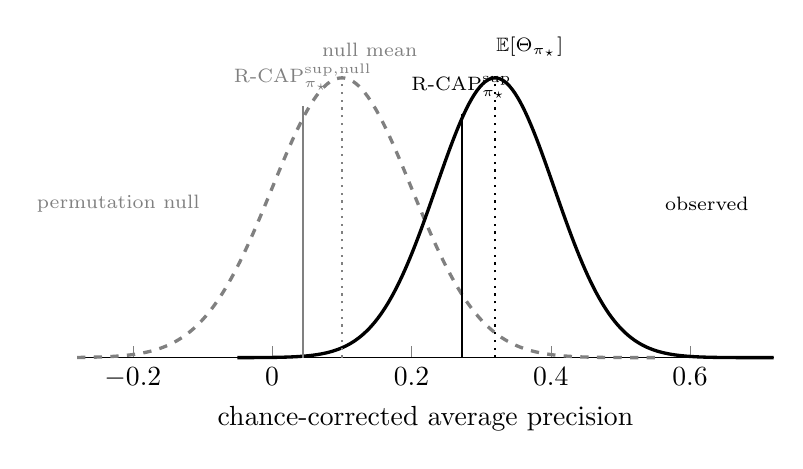
\begin{tikzpicture}
\begin{axis}[
  width=0.86\textwidth, height=6.2cm,
  xlabel={chance-corrected average precision},
  xmin=-0.28, xmax=0.72,
  ymin=0, ymax=1.30,
  axis y line=none,
  axis x line*=bottom,
  xtick={-0.2,0,0.2,0.4,0.6},
  clip=false,
  every axis plot/.append style={very thick},
]
% null replication distribution
\addplot[dashed, gray, domain=-0.28:0.55, samples=200]
  {exp(-((x-0.10)^2)/(2*0.100^2))};
% observed replication distribution
\addplot[solid, black, domain=-0.05:0.72, samples=200]
  {exp(-((x-0.32)^2)/(2*0.085^2))};
% markers
\draw[gray, dotted, thick] (axis cs:0.100,0) -- (axis cs:0.100,1.02);
\draw[gray, thick] (axis cs:0.044,0) -- (axis cs:0.044,0.90);
\draw[black, dotted, thick] (axis cs:0.320,0) -- (axis cs:0.320,1.02);
\draw[black, thick] (axis cs:0.272,0) -- (axis cs:0.272,0.87);
\node[gray, font=\scriptsize, anchor=south] at (axis cs:0.044,0.92) {$\RCAPnull$};
\node[gray, font=\scriptsize, anchor=south] at (axis cs:0.14,1.04) {null mean};
\node[font=\scriptsize, anchor=south] at (axis cs:0.272,0.89) {$\RCAP$};
\node[font=\scriptsize, anchor=south] at (axis cs:0.37,1.04) {$\E[\Theta_{\pi_\star}]$};
\node[gray, font=\scriptsize, anchor=east] at (axis cs:-0.09,0.55) {permutation null};
\node[font=\scriptsize, anchor=west] at (axis cs:0.55,0.55) {observed};
\end{axis}
\end{tikzpicture}
\caption{Estimated replication distributions for the observed evaluation (solid) and the conditional permutation null (dashed), each summarized by its mean and by $S_2$, which sits below the mean by the disagreement penalty. The null lies above zero, a common result at small positive counts.}
\label{fig:distribution}
\end{figure}

Beyond the four quantities of Table~\ref{tab:ladder} and the permutation $p$-value, a complete report states $\pi_\star$, the observed class counts and the class-count design of each replicate, the declared regime, the method and exchangeable unit used to generate replicates and to permute outcomes, the counts $B$ and $M$ with the Monte Carlo stability criterion, and how the predictions were separated from the outcomes used for evaluation. The following paragraph reports all of them.
\begin{quote}
At a reference prevalence of $0.10$, R-CAP was $0.247$. The supported effect $\widehat{\operatorname{R\text{-}CAP}}{}^{\,\mathrm{sup}}_{0.10}$ was $0.270$, and expected repeated performance was $0.298$, giving a disagreement penalty of $0.028$. The conditional permutation null was $0.031$, with $p<0.002$. The calibrated scale places this conditional chance level at zero and perfect separation at one. The observed chance-corrected average precision $\CAP_{0.10}(D_{\mathrm{obs}})$ was $0.340$. The held-out evaluation contained 100 positive and 900 negative patients. Each of $5{,}000$ stratified bootstrap replicates sampled 100 positive and 900 negative patients with replacement from their observed classes. The null held the score vector fixed and used $500$ outcome permutations across patients, each followed by the same $5{,}000$-replicate procedure. Doubling $B$ and $M$ left both supported estimates stable to three decimal places.
\end{quote}

If the supported effect does not clear its conditional null, omit the calibrated headline. Report the result as at or below measured chance, give both supported quantities and the permutation $p$-value, and read direction from the signed observed effect in Equation~\eqref{eq:T}.

When no single target prevalence is scientifically privileged, report
\[
\pi_\star
\longmapsto
\left\{
\Tpi(D_{\mathrm{obs}}),
\RCAPHat
\right\}
\]
over a prespecified plausible range, as in Figure~\ref{fig:profile}. This profile shows whether performance levels, disagreement penalties, or model orderings depend materially on the reference population.

\begin{figure}[ht]
\centering
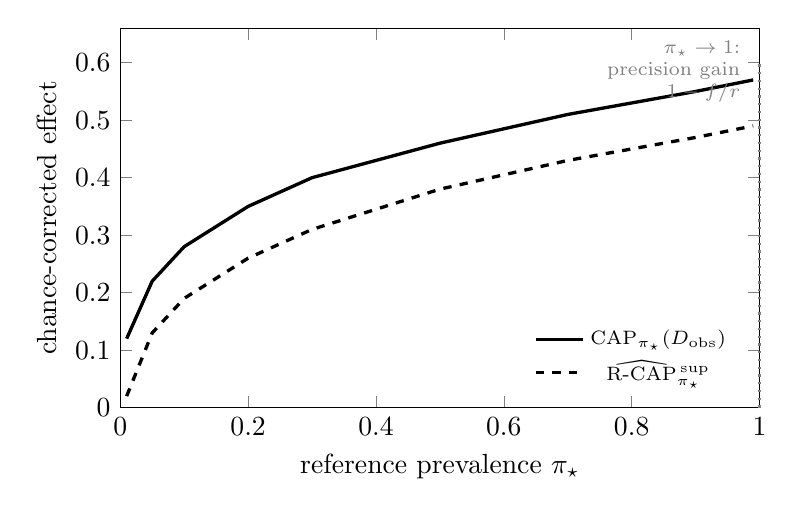
\begin{tikzpicture}
\begin{axis}[
  width=0.80\textwidth, height=6.4cm,
  xlabel={reference prevalence $\pi_\star$},
  ylabel={chance-corrected effect},
  xmin=0, xmax=1.0,
  ymin=0, ymax=0.66,
  xtick={0,0.2,0.4,0.6,0.8,1.0},
  ytick={0,0.1,0.2,0.3,0.4,0.5,0.6},
  legend pos=south east,
  legend style={font=\scriptsize, draw=none, fill=none},
  every axis plot/.append style={very thick},
  clip=false,
]
\addplot[black, mark=none] coordinates {
 (0.01,0.12) (0.05,0.22) (0.10,0.28) (0.20,0.35) (0.30,0.40)
 (0.50,0.46) (0.70,0.51) (0.90,0.55) (0.99,0.57)};
\addlegendentry{$\Tpi(D_{\mathrm{obs}})$}
\addplot[black, dashed, mark=none] coordinates {
 (0.01,0.02) (0.05,0.13) (0.10,0.19) (0.20,0.26) (0.30,0.31)
 (0.50,0.38) (0.70,0.43) (0.90,0.47) (0.99,0.49)};
\addlegendentry{$\RCAPHat$}
\draw[gray, dotted, thick] (axis cs:1.0,0) -- (axis cs:1.0,0.60);
\node[gray, font=\scriptsize, anchor=north east, align=right]
  at (axis cs:0.985,0.655) {$\pi_\star\to1$:\\ precision gain\\ $1-f/r$};
\end{axis}
\end{tikzpicture}
\caption{Illustrative reference-prevalence profile for one model. The observed effect and its supported counterpart are both nondecreasing in $\pi_\star$ for a better-than-chance ranker, by Equation~\eqref{eq:reference-prevalence-derivative}, and the disagreement penalty is largest where small changes in empirical false-positive rates matter most. The right-hand edge marks the limit at which the threshold-level integrand coincides with prevalence-free precision gain, per Section~\ref{sec:related-normalizations}. Values are illustrative.}
\label{fig:profile}
\end{figure}

\section{How evaluation size enters R-CAP\textsuperscript{sup}}

Return to two observed evaluations with chance-corrected average precision near $0.30$. Under the canonical estimator, the evaluation with 20 positive cases produces bootstrap repetitions containing 20 positives, while the evaluation with 20,000 positive cases produces repetitions containing 20,000 positives. Each also preserves its observed negative count. Table~\ref{tab:illustration} illustrates replication distributions with the same mean repeated effect.

\begin{table}[ht]
\centering
\caption{Illustrative same-design repetitions with the same mean repeated effect.}
\label{tab:illustration}
\begin{tabular}{@{}lccc@{}}
\toprule
Evaluation & $\E[\Theta_{\pi_\star}]$ & $\tfrac12\E|\Theta_{\pi_\star,1}-\Theta_{\pi_\star,2}|$ & R-CAP\textsuperscript{sup} \\
\midrule
20 positive cases & $0.30$ & $0.12$ & $0.18$ \\
20,000 positive cases & $0.30$ & $0.01$ & $0.29$ \\
\bottomrule
\end{tabular}
\end{table}

The smaller evaluation loses more of its repeated effect, since individual positive ranks carry greater influence and its repetitions disagree more. The values are illustrative, and a validation study must characterize this behavior under specified score distributions.

Evaluation size also moves the chance level. The smaller design can have a larger disagreement penalty under permutation and a larger upward AP bias. Calibration subtracts their net contribution as measured by the conditional null.

R-CAP\textsuperscript{sup} contains no multiplicative sample-size factor. Positive and negative counts affect the score through the replication distribution induced by the repeated-evaluation design. As that distribution contracts around a value $t_0$,
\[
\RCAP\longrightarrow t_0.
\]
Additional information can reduce the disagreement penalty while leaving the limiting average-precision scale unchanged.

\section{Mathematical behavior and interpretive limits}
\label{sec:properties}

\subsection{Basic properties}

A perfectly stable regime leaves no penalty: if $\Theta_{\pi_\star}=t$ almost surely then $\RCAP=t$. The supported score never exceeds mean repeated performance, and it inherits the bounds of its argument, so $\RCAP$ lies in $[-\pi_\star/(1-\pi_\star),\,1]$ for Equation~\eqref{eq:T}. A replication distribution that dominates another in the first-order stochastic sense has the larger R-CAP\textsuperscript{sup}. Appendix~\ref{app:properties} proves these, gives a quantile representation, and identifies $S_2$ within two established families.

The penalty depends on the whole replication distribution. Two distributions sharing a mean and a variance can assign different probability to lower-tail failures and take different R-CAP\textsuperscript{sup} values.

\subsection{What the reported value does not carry}
\label{sec:collision}

The other direction matters more. Equation~\eqref{eq:decomposition} subtracts, and a difference cannot report its operands.

\begin{table}[ht]
\centering
\caption{Two replication distributions with the same supported effect.}
\label{tab:collision}
\begin{tabular}{@{}lccc@{}}
\toprule
Replication distribution & $\E[\Theta_{\pi_\star}]$ & penalty & R-CAP\textsuperscript{sup} \\
\midrule
$0.9$ and $0.1$ with equal probability & $0.500$ & $0.200$ & $0.300$ \\
$0.3$ with probability one & $0.300$ & $0.000$ & $0.300$ \\
\bottomrule
\end{tabular}
\end{table}

The first design is a coin flip between a strong result and a weak one. The second returns the same middling value every repetition. They report the same headline.

Section~\ref{sec:reporting} requires $\widehat{\E}[\Theta_{\pi_\star}]$ for this reason. Equation~\eqref{eq:decomposition} is an identity, so any two of its three quantities fix the third. Read as mean and penalty, the first design is $(0.500,0.200)$ and the second $(0.300,0.000)$.

Two numbers still do not determine a distribution. For an equiprobable three-point replication distribution the penalty depends only on the range, so sliding the support with its range and sum held fixed moves the lower tail while the mean and the penalty stay where they are.

\begin{table}[ht]
\centering
\caption{Two replication distributions agreeing on the whole of Equation~\eqref{eq:decomposition} and differing in the lower tail.}
\label{tab:collision-tail}
\begin{tabular}{@{}lcccc@{}}
\toprule
Equiprobable support & $\E[\Theta_{\pi_\star}]$ & penalty & R-CAP\textsuperscript{sup} & $m_{0.5}$ \\
\midrule
$\{0.0,\,0.6,\,0.6\}$ & $0.400$ & $0.133$ & $0.267$ & $0.00$ \\
$\{0.2,\,0.2,\,0.8\}$ & $0.400$ & $0.133$ & $0.267$ & $0.20$ \\
\bottomrule
\end{tabular}
\end{table}

The first fails outright in one repetition of three. The second never falls below $0.2$. Section~\ref{sec:survival} reads that difference through the survival level $m_\gamma$, which is the summary to add whenever the lower tail is the decision.

\subsection{Relation to a standard-error adjustment}

For a replication distribution that is approximately normal with standard deviation $\sigma$, $\E|\Theta_1-\Theta_2|=2\sigma/\sqrt{\pi}$, so
\begin{equation}
\RCAP
\approx
\E[\Theta_{\pi_\star}]-\frac{\sigma}{\sqrt{\pi}}
\approx
\E[\Theta_{\pi_\star}]-0.564\,\sigma .
\label{eq:se-approximation}
\end{equation}
To first order the estimate is the mean repeated effect shifted down by slightly more than half a replication standard deviation, roughly the $29$th percentile under normality. It serves as a check.

The exact minimum form requires no distributional assumption. The constant $0.564$ applies only under normality and can misstate the penalty for skewed or discrete replication distributions. Sparse positives and heavy ties often produce those shapes. The same operator also applies to paired differences without a separate correlation adjustment. Its population target requires a finite first moment.

The supported score and an uncertainty interval answer different questions. Section~\ref{sec:reporting} gives the estimate, and Section~\ref{sec:error} gives its uncertainty.

\subsection{Monte Carlo error and estimation error}
\label{sec:error}

$\RCAPHatB$ has Monte Carlo error from finite $B$ and estimation error from using $\PRepHat$ in place of $\PRep$.

Equation~\eqref{eq:uestimator} is a U-statistic of degree two. Its leading Monte Carlo variance is governed by the Hoeffding projection $h_1(t)=\E[\min(t,\Theta_{\pi_\star})]$~\cite{hoeffding1948ustat}. A leave-one-out estimate on the sorted replicate array is
\begin{equation}
\widehat h_{1,-i}(t_{(i)})
=
\frac{1}{B-1}
\left\{
\sum_{j<i}t_{(j)}
+
(B-i)\,t_{(i)}
\right\},
\qquad
\widehat{\operatorname{se}}_{\mathrm{MC}}
=
\frac{2}{\sqrt{B}}
\operatorname{sd}_{1\leq i\leq B}
\{\widehat h_{1,-i}(t_{(i)})\}.
\label{eq:mcse}
\end{equation}
Equation~\eqref{eq:mcse} is a first-order standard error. Finite-$B$ corrections are of smaller order. The calculation uses one prefix sum over an array the estimator has already sorted and falls at rate $B^{-1/2}$.

Increasing $B$ leaves estimation error unchanged. That error is governed by the evaluation units and their class counts. A nested bootstrap measures it by resampling evaluation units in an outer loop and running the complete estimator within each outer dataset. Influence-function methods for L-moments give an analytic alternative when their large-sample approximation is credible~\cite{hosking1990lmoments}. Section~\ref{sec:superiority} uses this outer loop to bound supported superiority in a paired comparison.

The calibrated score also contains Monte Carlo error from estimating $\RCAPnullHat$. A delta-method calculation may use independent random streams for $\RCAPHat$ and $\RCAPnullHat$. Shared random numbers require their covariance. Report the first-order Monte Carlo errors routinely. A conclusion that turns on the distance from the conditional null should also report the nested-bootstrap spread.

\subsection{The support distribution and a survival level}
\label{sec:survival}

The support distribution has a simple form. Let $F$ be the distribution function of $\Theta_{\pi_\star}$ and $Q_{\pi_\star}$ its quantile function. Two independent repetitions give
\[
\Pr(M>m)=\{1-F(m)\}^2,
\qquad
M=\min\{\Theta_{\pi_\star,1},\Theta_{\pi_\star,2}\}.
\]
The level retained by both repetitions with frequency $\gamma$ is
\begin{equation}
m_\gamma=Q_{\pi_\star}(1-\sqrt{\gamma}).
\label{eq:survival-level}
\end{equation}
R-CAP\textsuperscript{sup} is the mean of $M$, and $m_\gamma$ is a low quantile of the same distribution. Under an approximately normal replication distribution the two track each other and R-CAP\textsuperscript{sup} sits near $m_{0.5}$. They separate when the distribution is lumpy. For a regime returning $\Theta_{\pi_\star}=1$ with probability $0.9$ and $0$ otherwise, R-CAP\textsuperscript{sup} is $0.81$ while $m_{0.9}$ is $0$. The gap $\RCAP-m_\gamma$ measures how much of the retained level depends on repetitions that can fail, and it is largest in the sparse-positive designs of Section~\ref{sec:sparse}.

The estimate is one index into the sorted replicate array of Appendix~\ref{app:computation},
\[
\widehat m_\gamma
=
t_{\left(\max\{1,\lceil B(1-\sqrt{\gamma})\rceil\}\right)}.
\]
It is a quantile of the estimated replication distribution and has the same status as $\RCAPHat$. It is not a confidence bound for a population parameter. A tail quantile is noisier than the mean and needs a larger $B$, and its estimate is least reliable in the sparse-positive regime where it is most informative. For general $K$ the same argument gives $m_\gamma^{(K)}=Q_{\pi_\star}(1-\gamma^{1/K})$, so $K$ and $\gamma$ traverse the same tail.

\subsection{Random ranking and the calibrated zero}

The chance-corrected effect $\Tpi$ places population random ranking at zero, and the support functional retains the finite-sample residual of Equation~\eqref{eq:two-distortions}. For fixed predictions, Equation~\eqref{eq:conditional-null} measures that residual and Equation~\eqref{eq:calibrated} removes it.

The signed score preserves below-chance information. Clipping at zero changes finite-sample behavior near chance and should be avoided.

\subsection{Dependence on the reference prevalence}

Changing $\pi_\star$ changes the effect assigned to each repeated dataset and with it the center, shape, and lower tail of the replication distribution. A low reference prevalence makes early false positives especially influential, and the resulting effect on disagreement depends on the score distributions, class counts, ties, and dependence structure. The permutation null must be recomputed at each $\pi_\star$ for which a calibrated value is reported. Since model rankings can reverse across $\pi_\star$, a claim of greater supported performance should state the reference prevalence or the range over which the ordering holds.

\subsection{Dependence on the declared regime}

$\RCAP$ is conditional on the declaration of Section~\ref{sec:regime}. Widening the environment set or releasing a mechanism changes the question being answered. Sensitivity analysis can compare plausible declarations, and external replication tests whether the stated invariances survive changes in site, time, instrument, or population composition. The name replication-adjusted describes the operator and says nothing about the breadth of the regime, so a value carries external meaning only when the declared environment set spans the changes at issue.

\subsection{Sparse positive cases}
\label{sec:sparse}

Small positive counts make AP discrete and sensitive to individual ranks. They also limit empirical estimation of the positive score distribution, and they inflate both terms in Equation~\eqref{eq:two-distortions}. A low estimated R-CAP\textsuperscript{sup} can reflect weak repeated performance, broad variation across repetitions, limited information for estimating $\PRep$, or a combination of these features. Reporting $\RCAPnullHat$ shows what the same pipeline retains after the observed association has been removed. Its tail rests on the same small positive count, so the benchmark is least reliable where the supported level is hardest to estimate.

\subsection{Replication count and severity}

The replication count $K$ sets how many independent repetitions a performance claim must survive. It is a severity parameter of the same kind as the declared regime and the reference prevalence, and it is declared with them. A stronger criterion uses
\[
S_K
=
\E\left[
\min(\Theta_{\pi_\star,1},\ldots,\Theta_{\pi_\star,K})
\right],
\]
which asks the claim to survive $K$ repetitions and places greater weight on the lower tail. Appendix~\ref{app:properties} gives the corresponding quantile weight. $S_K$ is decreasing in $K$ for any nondegenerate distribution, which is the content of the criterion: a claim asked to survive more repetitions is corroborated at a lower level.

The strict version asks a claim to survive every repetition the regime can produce. That level is $\lim_{K\to\infty}S_K$, the essential infimum of $\Theta_{\pi_\star}$. A finite sample cannot estimate it, since it estimates as the worst replicate and does not stabilize. Corroboration in practice is relative to a finite number of tests, and $K$ names that number. The default $K=2$ is the smallest count that expresses a repeated-performance criterion. Larger $K$ states a stricter claim and must be prespecified.

\subsection{Centering}

The definition in Equation~\eqref{eq:rcap} is replication-centered. A data-centered alternative preserves the observed point estimate and subtracts only the estimated penalty. Appendix~\ref{app:centering} states both forms and the grounds for preferring the first.

\section{Paired comparisons and other performance effects}
\label{sec:paired}

\subsection{Paired model comparison}

Suppose models $A$ and $B$ are evaluated on the same execution $D^{\mathrm{rep}}$ of the declared regime. Some repeated datasets may be easier for both models, while others may be harder. Their comparative performance within one evaluation is
\begin{equation}
\Delta_{\pi_\star}
=
\CAP_{A,\pi_\star}(D^{\mathrm{rep}})
-
\CAP_{B,\pi_\star}(D^{\mathrm{rep}}).
\label{eq:paired-difference}
\end{equation}
A positive value favors model $A$, a negative value favors model $B$, and zero represents equal chance-corrected average precision at reference prevalence $\pi_\star$.

Two independent executions of the regime produce
\[
\Delta_{\pi_\star,1},
\Delta_{\pi_\star,2}
\iid
P_{\mathrm{rep}}^{\Regime,\Delta_{\pi_\star}}.
\]
A superiority level $s$ is retained by both repetitions when
\[
s\leq \Delta_{\pi_\star,1},
\qquad
s\leq \Delta_{\pi_\star,2}.
\]
The largest such level is their minimum. Define supported superiority by
\begin{equation}
S_2(\Delta_{\pi_\star};\Regime)
=
\E_{\Regime}
\left[
\min\{
\Delta_{\pi_\star,1},
\Delta_{\pi_\star,2}
\}
\right].
\label{eq:paired}
\end{equation}
Using the minimum identity gives
\begin{equation}
S_2(\Delta_{\pi_\star};\Regime)
=
\E_{\Regime}[\Delta_{\pi_\star}]
-
\frac12
\E_{\Regime}
\left[
|\Delta_{\pi_\star,1}-\Delta_{\pi_\star,2}|
\right].
\label{eq:paired-decomposition}
\end{equation}
The first term is the expected advantage of model $A$ across repeated evaluations. The second term is half the expected disagreement between repeated advantages. A positive value retains a positive advantage for model $A$ under the two-repetition criterion. A nonpositive value supplies no positive supported-superiority claim for model $A$.

For estimation, evaluate both models on every replicated dataset $D^{(b)}$. Define
\[
t_{A,b}=\CAP_{A,\pi_\star}(D^{(b)}),
\qquad
t_{B,b}=\CAP_{B,\pi_\star}(D^{(b)}),
\qquad
\delta_b=t_{A,b}-t_{B,b}.
\]
The same resampled evaluation units and outcomes are used for both models within replicate $b$. This preserves the pairing and allows shared changes in evaluation difficulty to cancel in $\delta_b$. The all-pairs estimator is
\begin{equation}
\widehat S_{2,B}(\Delta_{\pi_\star};\Regime)
=
\frac{2}{B(B-1)}
\sum_{1\leq i<j\leq B}
\min(\delta_i,\delta_j).
\label{eq:paired-estimator}
\end{equation}

Identical rankings give $\delta_b=0$ in every replicate. Models with different score structures can retain a nonzero supported difference under joint no-signal outcomes, because their finite-sample AP biases differ.

\subsection{Inference for supported superiority}
\label{sec:superiority}

Calibration of a single model uses a sharp null because a suitable one exists. The hypothesis $Y\perp S$ states exactly what the calibrated zero represents, that the realized scores carry no outcome information, and permuting outcomes against fixed scores generates its reference distribution without approximation.

No sharp hypothesis plays that role for a comparison. Two models can both carry substantial signal while performing equally, so a hypothesis that removes all signal does not express equality of performance. Two models can also differ in score structure, in which case neither is exchangeable with the other and their labels cannot be permuted. Inference for superiority therefore targets the estimand directly.

The substantive claim is that model $A$ retains an advantage under repeated evaluation,
\[
S_2(\Delta_{\pi_\star};\Regime)>0,
\]
so the falsification target is
\[
H_0^{\mathrm{sup}}:
S_2(\Delta_{\pi_\star};\Regime)\leq 0 .
\]
This hypothesis contains equal performance, superiority of model $B$, and advantages of model $A$ too unstable across repetitions to survive the two-repetition criterion.

Equation~\eqref{eq:paired-decomposition} shows how demanding the claim is. Under equal performance $\E_{\Regime}[\Delta_{\pi_\star}]=0$, so
\[
S_2(\Delta_{\pi_\star};\Regime)
=
-\tfrac12\E_{\Regime}\left[|\Delta_{\pi_\star,1}-\Delta_{\pi_\star,2}|\right]
<
0
\]
for any nondegenerate replication distribution of the difference. Equal performance lies strictly inside the null rather than on its boundary. The boundary requires
\[
\E_{\Regime}[\Delta_{\pi_\star}]
=
\tfrac12
\E_{\Regime}\left[|\Delta_{\pi_\star,1}-\Delta_{\pi_\star,2}|\right],
\]
so model $A$ must exceed model $B$ on average by more than half the expected disagreement between repeated advantages before any positive supported superiority is claimed. This is the replication criterion applied to the comparison.

Evidence against $H_0^{\mathrm{sup}}$ takes the form of a lower confidence bound for $S_2(\Delta_{\pi_\star};\Regime)$ lying above zero. The Monte Carlo standard error of Equation~\eqref{eq:mcse} does not supply one. That quantity describes the accuracy of the all-pairs average at fixed $\PRepHat$, and increasing $B$ drives it toward zero while leaving the relevant uncertainty unchanged.

The bound requires the outer resampling procedure of Section~\ref{sec:error}. The estimate then has two nested loops with distinct roles. The inner loop generates the replication distribution declared by the regime and defines the estimand. The outer loop resamples evaluation units and measures how well one evaluation pins that estimand down. Report the outer spread with the point estimate whenever a conclusion turns on the sign of $S_2(\Delta_{\pi_\star};\Regime)$.

Two cautions attach to the bound. The replication distribution of $\Delta_{\pi_\star}$ is skewed by the disagreement penalty, so a studentized or bias-corrected and accelerated interval is preferable to a percentile interval. And $S_2$ averages a kernel that is nondifferentiable where its arguments coincide. The expectation smooths that kink when the replication distribution of the difference is continuous, and the smoothing weakens when the difference is discrete and lumpy. Sparse positive counts and heavy ties produce that shape, as Section~\ref{sec:sparse} describes, and those designs are also the ones in which $\Delta_{\pi_\star}$ concentrates near zero. Coverage should be treated as unverified there until simulation establishes it.

The null is relative to the declared regime. As the replication distribution contracts, $S_2(\Delta_{\pi_\star};\Regime)$ rises toward $\E_{\Regime}[\Delta_{\pi_\star}]$ from below, so a larger evaluation raises the estimand while also tightening the bound around it. Rejecting $H_0^{\mathrm{sup}}$ establishes supported superiority under the evaluation design that was declared, and that design belongs in the statement of the result.

\subsection{An optional joint no-signal benchmark}
\label{sec:joint-null}

A separate question asks how much supported advantage the two score structures generate when neither carries outcome information. Let $\mathbf{s}_A$ and $\mathbf{s}_B$ be the realized score vectors on the same evaluation units. Condition on both and permute one outcome vector jointly against the pair. For each permutation, use the same resampled units for both models, calculate the replicate differences, and apply $S_2$ to those differences. Outcomes are permuted at the original exchangeable unit, and bootstrap replicates remain Monte Carlo draws from each permuted evaluation.

The sharp hypothesis is
\[
Y\perp(S_A,S_B),
\]
which says that neither fixed score vector carries outcome information. If $\widehat S_{2,B}^{\Delta,(m)}$ is the supported difference from permutation $m$, report its mean and
\[
p_\Delta
=
\frac{
1+\#\{m:\widehat S_{2,B}^{\Delta,(m)}
\geq \widehat S_{2,B}(\Delta_{\pi_\star};\Regime)\}
}{M+1}.
\]

Report $p_\Delta$ only as a test of $Y\perp(S_A,S_B)$. Its value is diagnostic: it measures the supported advantage produced by the differing finite-sample AP biases of the two score structures once the common outcome association has been removed. It is not a test of superiority. When both models are credible predictors the joint hypothesis is easy to reject, and rejecting it says little about whether $A$ outperforms $B$. Inference about superiority uses $H_0^{\mathrm{sup}}$ of Section~\ref{sec:superiority}.

\subsection{Marginal values cannot be differenced}

Subtracting two marginal R-CAP\textsuperscript{sup} values gives something else, and the direction of the discrepancy is fixed.

\begin{proposition}[Marginals overstate supported superiority]
Let $\CAP_{A,\pi_\star}$ and $\CAP_{B,\pi_\star}$ have finite first moments under $\Regime$, with any joint law. Then
\[
S_2(\CAP_{A,\pi_\star};\Regime)
-
S_2(\CAP_{B,\pi_\star};\Regime)
\;\geq\;
S_2(\Delta_{\pi_\star};\Regime),
\]
with equality if and only if $\CAP_{B,\pi_\star}$ and $\Delta_{\pi_\star}$ are comonotone.
\end{proposition}

\begin{proof}
Equation~\eqref{eq:quantile} represents $S_2$ as a distortion measure with distortion $g(u)=1-(1-u)^2$, which is concave. A concave distortion is superadditive on gains, $S_2(X+Y)\geq S_2(X)+S_2(Y)$, with equality exactly when $X$ and $Y$ are comonotone; Appendix~\ref{app:families} records both facts. Apply superadditivity to $\CAP_{A,\pi_\star}=\CAP_{B,\pi_\star}+\Delta_{\pi_\star}$ and rearrange.
\end{proof}

Differencing marginals therefore never understates model $A$'s supported advantage, and it reports the paired quantity exactly when $A$'s advantage rises and falls with $B$'s performance across the regime. When the advantage is largest where the baseline is weakest, the two diverge. Consider a regime with two equally likely evaluation contexts:
\begin{center}
\begin{tabular}{@{}lccc@{}}
\toprule
Context & $\CAP_{A,\pi_\star}$ & $\CAP_{B,\pi_\star}$ & $\Delta_{\pi_\star}$ \\
\midrule
1 & $0.90$ & $0.80$ & $0.10$ \\
2 & $0.40$ & $0.10$ & $0.30$ \\
\bottomrule
\end{tabular}
\end{center}
The paired difference takes values $0.10$ and $0.30$ with equal probability, which gives
\[
S_2(\Delta_{\pi_\star};\Regime)=0.15.
\]
The marginal support values are
\[
S_2(\CAP_{A,\pi_\star};\Regime)=0.525,
\qquad
S_2(\CAP_{B,\pi_\star};\Regime)=0.275,
\]
so their difference is $0.25$, above the paired value of $0.15$ as the proposition requires. Model $A$'s advantage is largest in the context where $B$ performs worst, which is the countermonotone case, and the gap between the two quantities is widest there. Subtracting marginal support values compares two separate replication summaries. Equation~\eqref{eq:paired} evaluates the advantage of model $A$ within each repeated dataset and then applies the support criterion to that advantage. It follows that marginal R-CAP\textsuperscript{sup} values reported in separate studies cannot be differenced to infer supported superiority; a paired comparison requires joint evaluation on common replicates.

\subsection{Other performance effects}

The operator in Equation~\eqref{eq:support-operator} can be applied to AUROC, correlation, $R^2$, subgroup contrasts, and paired improvements. The effect must be oriented so that larger values indicate better performance. For a loss $L(D)$, use $T(D)=-L(D)$. For comparison of two models by loss, use
\[
T(D)=L_B(D)-L_A(D),
\]
so positive values favor model $A$.

Each application needs a replication regime suited to its scientific claim. A conditional calibration also needs a sharp no-signal hypothesis and a declared exchangeable unit. Effects defined as contrasts, whether between two models or between two subgroups, follow Section~\ref{sec:superiority}, where the claim is a positive value of $S_2$ and the evidence is a lower bound above zero. These choices belong to the performance effect and the study design.

\section{Conclusion}

Three declarations fix what this paper reports, and each is a scientific choice rather than a technical default.

The reference prevalence $\pi_\star$ names the population in which selected-set purity is read. Precision odds factor into prior odds and a likelihood ratio, so prevalence enters through one term alone; declaring $\pi_\star$ replaces that term, where prevalence-free normalizations divide it out. Chance correction then places random ranking at zero and perfect ranking at one, giving $\Tpi(D)$. When several target populations are relevant, a reference-prevalence profile accompanies the primary value.

The evaluation-generating regime $\Regime$ names the environments a repetition may visit and the mechanisms held invariant across them, of which $\pi_\star$ is one instance applied to the class prior. On that regime the support operator
\[
S_2(T;\Regime)
=
\E_{\Regime}\left[\min(T_1,T_2)\right]
\]
returns the performance level two independent executions retain, for any effect $T$ oriented so that larger is better. Applied to $\CAP_{\pi_\star}$ it gives R-CAP\textsuperscript{sup}, equal to expected repeated performance minus half the expected disagreement between repetitions. The quantity therefore depends jointly on the performance functional, the reference population, and the regime. Applied instead to within-replication differences it measures supported superiority of one model over another, which differencing marginal values overstates and which is established by a lower bound above zero rather than by a no-signal permutation.

The conditional null names what chance means for the predictions at hand. Analytic chance correction leaves a finite-sample residual, since non-interpolated average precision is biased upward under random ranking while the minimum imposes a downward penalty. For fixed predictions on development-independent outcomes, permuting outcomes against the realized scores measures that residual while preserving the score distribution and ties, and
\[
\RCAPcalHat
=
\frac{\RCAPHat-\RCAPnullHat}{1-\RCAPnullHat}
\]
places it at zero with perfect separation at one. The canonical stratified bootstrap attains that upper anchor exactly when the observed scores separate the classes, so ties mixing outcomes lower the supported effect and leave the anchor fixed, charging loss of score resolution to performance. The observed effect, expected repeated performance, supported effect, conditional null, and permutation $p$-value are reported with the calibrated value, since each adjustment separating them is then visible.

What remains open is empirical. Simulation and applied study are needed on finite-sample behavior, sensitivity to sparse positives, robustness to misdeclared regimes, coverage of the superiority bound, and the adequacy of the canonical bootstrap. A regime that repeats model development can define and estimate $S_2$ but needs its own null before a calibrated value is available. The proposal supplies a population support target, an estimator for the common fixed-model setting, and a conditional no-association benchmark for the predictions actually evaluated.

\newpage

\begin{thebibliography}{9}

\bibitem{bouckaert2004estimating}
Bouckaert, R. R. (2004).
Estimating replicability of classifier learning experiments.
In \emph{Proceedings of the 21st International Conference on Machine Learning}, pages 137--144.

\bibitem{elkan2001foundations}
Elkan, C. (2001).
The foundations of cost-sensitive learning.
In \emph{Proceedings of the 17th International Joint Conference on Artificial Intelligence}, pages 973--978.

\bibitem{flach2015prg}
Flach, P. A. and Kull, M. (2015).
Precision-Recall-Gain curves: PR analysis done right.
In Cortes, C., Lawrence, N. D., Lee, D. D., Sugiyama, M., and Garnett, R., editors,
\emph{Advances in Neural Information Processing Systems 28}, pages 838--846.

\bibitem{hoeffding1948ustat}
Hoeffding, W. (1948).
A class of statistics with asymptotically normal distribution.
\emph{Annals of Mathematical Statistics}, 19(3):293--325.

\bibitem{hosking1990lmoments}
Hosking, J. R. M. (1990).
L-moments: analysis and estimation of distributions using linear combinations of order statistics.
\emph{Journal of the Royal Statistical Society, Series B}, 52(1):105--124.

\bibitem{mayo1996error}
Mayo, D. G. (1996).
\emph{Error and the Growth of Experimental Knowledge}.
University of Chicago Press.

\bibitem{nadeau2003inference}
Nadeau, C. and Bengio, Y. (2003).
Inference for the generalization error.
\emph{Machine Learning}, 52(3):239--281.

\bibitem{ojala2010permutation}
Ojala, M. and Garriga, G. C. (2010).
Permutation tests for studying classifier performance.
\emph{Journal of Machine Learning Research}, 11:1833--1863.

\bibitem{popper1959logic}
Popper, K. R. (1959).
\emph{The Logic of Scientific Discovery}.
Hutchinson, London.

\bibitem{wang1996premium}
Wang, S. S. (1996).
Premium calculation by transforming the layer premium density.
\emph{ASTIN Bulletin}, 26(1):71--92.

\end{thebibliography}

\addtocontents{toc}{\protect\setcounter{tocdepth}{0}}

\newpage
\appendix

\section{Reference-prevalence average precision}
\label{app:prevalence}

\subsection{Population transformation}

Let $Y\in\{0,1\}$ be the outcome and let $S$ be a ranking score. At threshold $c$, define
\[
r(c)=\Pr(S\geq c\mid Y=1),
\qquad
f(c)=\Pr(S\geq c\mid Y=0).
\]
These quantities are the true-positive and false-positive rates. For prevalence $\pi$, precision is
\[
p_{\pi}(c)
=
\frac{\pi r(c)}{\pi r(c)+(1-\pi)f(c)}.
\]

Suppose an evaluation has prevalence $\pi$ and threshold-specific precision $p(c)$. The precision implied by reference prevalence $\pi_\star$ is
\begin{equation}
p_{\pi_\star}(c)
=
\frac{(\pi_\star/\pi)p(c)}
{(\pi_\star/\pi)p(c)
+
\{(1-\pi_\star)/(1-\pi)\}\{1-p(c)\}}.
\label{eq:precision-transform}
\end{equation}

The transformation keeps $r(c)$ and $f(c)$ fixed. It changes the class prior used to calculate precision. In odds form it is a single multiplication,
\[
\frac{p_{\pi_\star}}{1-p_{\pi_\star}}
=
\frac{\pi_\star(1-\pi)}{\pi(1-\pi_\star)}
\cdot
\frac{p}{1-p},
\]
which is Equation~\eqref{eq:odds} with the prior odds exchanged.

\subsection{Precision gain and the prevalence-free limit}
\label{app:precg}

Let $\operatorname{precG}=(p-\pi)/\{(1-\pi)p\}$ with $p=\pi r/\{\pi r+(1-\pi)f\}$ and write $D=\pi r+(1-\pi)f$. Then
\[
p-\pi
=
\frac{\pi r-\pi D}{D}
=
\frac{\pi\{r-\pi r-(1-\pi)f\}}{D}
=
\frac{\pi(1-\pi)(r-f)}{D},
\qquad
(1-\pi)p
=
\frac{(1-\pi)\pi r}{D},
\]
so
\[
\operatorname{precG}
=
\frac{\pi(1-\pi)(r-f)/D}{(1-\pi)\pi r/D}
=
\frac{r-f}{r}
=
1-\frac{f}{r}.
\]
The prevalence terms cancel identically. Comparing with Equation~\eqref{eq:precg-limit} confirms that precision gain is the $\pi_\star\to1$ limit of the threshold-level integrand used here.

The corresponding recall gain is $\operatorname{recG}=(r-\pi)/\{(1-\pi)r\}$, which vanishes at $r=\pi$ and equals one at $r=1$, with
\[
\frac{d\operatorname{recG}}{dr}
=
\frac{\pi}{(1-\pi)r^{2}} .
\]
Integrating precision gain against $d\operatorname{recG}$ therefore weights the region $r\in[\pi,1]$ proportionally to $r^{-2}$. Integrating the chance-corrected precision of Equation~\eqref{eq:threshold-normalized-effect} against $dr$ does not. The two summaries coincide at the threshold level in the limit and differ as integrals for every $\pi_\star$.

\subsection{Empirical definition}

Let
\[
D=\{(s_i,y_i)\}_{i=1}^{n},
\qquad y_i\in\{0,1\},
\]
with $n_+=\sum_i y_i>0$ and $n_-=n-n_+>0$. Let
\[
c_1>c_2>\cdots>c_K
\]
be the distinct observed score values. Threshold $k$ selects every observation with $s_i\geq c_k$. Define
\[
\operatorname{TP}_k
=
\sum_{i=1}^{n}\mathbf{1}\{y_i=1,\ s_i\geq c_k\},
\qquad
\operatorname{FP}_k
=
\sum_{i=1}^{n}\mathbf{1}\{y_i=0,\ s_i\geq c_k\},
\]
and
\[
r_k=\frac{\operatorname{TP}_k}{n_+},
\qquad
f_k=\frac{\operatorname{FP}_k}{n_-}.
\]
Reference-prevalence precision at the threshold is
\begin{equation}
p_{\pi_\star,k}
=
\frac{\pi_\star r_k}
{\pi_\star r_k+(1-\pi_\star)f_k}.
\label{eq:empirical-reference-precision}
\end{equation}
Set $r_0=0$. Reference-prevalence average precision is
\begin{equation}
\AP_{\pi_\star}(D)
=
\sum_{k=1}^{K}
(r_k-r_{k-1})p_{\pi_\star,k}.
\label{eq:standardized-ap}
\end{equation}
A threshold that adds only negative cases has $r_k-r_{k-1}=0$. Its false positives still affect precision at later thresholds.

Equation~\eqref{eq:standardized-ap} evaluates precision at thresholds determined by the observed positions of positive cases. This is the source of the upward bias $\beta$ in Equation~\eqref{eq:two-distortions}, since those positions are favorably placed by chance more often than the population baseline implies.

\subsection{Equal scores}

Equal scores form one threshold block. Every observation in the block enters the selected set at the same threshold. This rule uses only distinctions made by the model.

Consider the scores and classes
\[
(0.90,+),\quad(0.70,+),\quad(0.70,-),\quad(0.20,-).
\]
An arbitrary ordering of the two middle cases can produce ordinary AP of $1$ or $5/6$. The model assigns them the same score. Under the block rule, both enter at threshold $0.70$. Precision is then $2/3$ and recall rises from $1/2$ to $1$. Equation~\eqref{eq:standardized-ap}, with the observed prevalence used as the reference prevalence, gives
\[
\AP
=
\frac12(1)+\frac12\left(\frac23\right)
=
\frac56.
\]
Use the model's unrounded numerical scores when they are available. Rounding before evaluation can create ties that were absent from the model output. Because the permutation null of Section~\ref{sec:calibration} preserves the score multiset, it also preserves the tie structure, and the resulting chance level reflects the ties actually present.

\subsection{Average-precision convention}

Equation~\eqref{eq:standardized-ap} uses non-interpolated stepwise average precision. Each increase in recall receives the precision at the threshold that produced it.

Trapezoidal PR area joins adjacent operating points with straight lines. Interpolated AP replaces the empirical precision sequence with a precision envelope. These conventions can give different finite-sample values, and they carry different chance levels. All R-CAP calculations in this document use the stepwise convention in Equation~\eqref{eq:standardized-ap}.

\subsection{Equivalent weighted implementation}

The same quantity can be calculated by assigning each observation the class weight
\begin{equation}
w_i
=
\begin{cases}
\pi_\star/n_+, & y_i=1,\\[4pt]
(1-\pi_\star)/n_-, & y_i=0.
\end{cases}
\label{eq:reference-weights}
\end{equation}
The positive weights sum to $\pi_\star$. The negative weights sum to $1-\pi_\star$. At threshold $k$, weighted precision is
\[
\frac{(\pi_\star/n_+)\operatorname{TP}_k}
{(\pi_\star/n_+)\operatorname{TP}_k
+
\{(1-\pi_\star)/n_-\}\operatorname{FP}_k}
=
p_{\pi_\star,k},
\]
and weighted recall is
\[
\frac{(\pi_\star/n_+)\operatorname{TP}_k}{\pi_\star}
=
r_k.
\]
A weighted AP routine therefore returns $\AP_{\pi_\star}(D)$ when it groups equal scores and uses non-interpolated stepwise AP.

Under the canonical stratified bootstrap, $n_+^{(b)}=n_+$ and $n_-^{(b)}=n_-$ for every replicate. Recalculate the threshold counts, $r_k^{(b)}$, and $f_k^{(b)}$ within each replicate while keeping $\pi_\star$ fixed. When the declared regime allows class counts to vary, use the replicate-specific $n_+^{(b)}$ and $n_-^{(b)}$ in the class weights. Each replicate must contain both outcome classes. A procedure that drops zero-class executions changes the regime-relative replication distribution and requires an explicit conditional estimand.

The prevalence transformation holds the class-conditional score mechanism invariant while the class prior moves to $\pi_\star$. Prior-probability shift is exactly that environment change. A change in the composition of either class alters the mechanism assumed invariant and voids the transformation, which is the failure mode of any regime whose declared invariance does not hold.

\section{Properties of the support functional}
\label{app:properties}

\subsection{Common support}

\begin{proposition}
For realized values $t_1$ and $t_2$, the largest real number that does not exceed either value is $\min(t_1,t_2)$.
\end{proposition}

\begin{proof}
Every admissible level $s$ satisfies $s\leq t_1$ and $s\leq t_2$, so $s\leq\min(t_1,t_2)$. The value $\min(t_1,t_2)$ satisfies both inequalities. It is therefore the largest admissible level.
\end{proof}

\subsection{Disagreement decomposition}

\begin{proposition}
If $\Theta_{\pi_\star,1}$ and $\Theta_{\pi_\star,2}$ are independent and identically distributed with finite first moment, then
\[
\E\min(\Theta_{\pi_\star,1},\Theta_{\pi_\star,2})
=
\E\Theta_{\pi_\star}
-
\frac12
\E|\Theta_{\pi_\star,1}-\Theta_{\pi_\star,2}|.
\]
\end{proposition}

\begin{proof}
Use
\[
\min(a,b)=\frac{a+b-|a-b|}{2}
\]
and take expectations. Identical distributions give
\[
\E\Theta_{\pi_\star,1}
=
\E\Theta_{\pi_\star,2}
=
\E\Theta_{\pi_\star}.
\]
\end{proof}

\subsection{Quantile representation}

Let $Q_{\pi_\star}(u)$ be a generalized quantile function of $\Theta_{\pi_\star}$. If $\E|\Theta_{\pi_\star}|<\infty$, then
\begin{equation}
S_K
=
\int_0^1 K(1-u)^{K-1}Q_{\pi_\star}(u)\,du,
\qquad
\RCAP
=
\int_0^1 2(1-u)Q_{\pi_\star}(u)\,du.
\label{eq:quantile}
\end{equation}

To see this, write $\Theta_{\pi_\star,i}=Q_{\pi_\star}(U_i)$ for independent $U_i\sim\operatorname{Uniform}(0,1)$. Since $Q_{\pi_\star}$ is nondecreasing,
\[
\min_i\{Q_{\pi_\star}(U_i)\}
=
Q_{\pi_\star}\{\min_i(U_i)\}.
\]
The minimum of $K$ independent uniform variables has density $K(1-u)^{K-1}$ on $(0,1)$.

Ordinary expectation weights quantiles uniformly. Equation~\eqref{eq:quantile} gives greater weight to lower quantiles through the $K$-repetition criterion, and the weighting becomes more concentrated on the lower tail as $K$ increases.

\subsection{Two established families}
\label{app:families}

The operator coincides with objects defined elsewhere, and the identification supplies several properties without separate proof.

\paragraph{L-moments.}
The first two L-moments of a distribution~\cite{hosking1990lmoments} are $\lambda_1=\E[T]$ and $\lambda_2=\tfrac12\E|T_1-T_2|$, the latter being half the Gini mean difference. Equation~\eqref{eq:general-decomposition} is therefore the exact identity
\[
S_2(T;\Regime)=\lambda_1-\lambda_2 .
\]
L-moment estimators are linear in order statistics, which is the origin of the sorted-sum form in Appendix~\ref{app:computation}, and they exist whenever the first moment does.

\paragraph{Distortion risk measures.}
Equation~\eqref{eq:quantile} expresses $S_K$ as a distortion measure with distortion function $g(u)=1-(1-u)^{K}$, a member of the dual-power family in the sense of Wang~\cite{wang1996premium}. Because $g$ is concave, the following hold immediately: monotonicity with respect to first-order stochastic dominance; monotonicity with respect to the concave order, so that a mean-preserving spread of the replication distribution cannot raise $S_2$; translation equivariance, $S_2(T+c)=S_2(T)+c$; positive homogeneity, $S_2(aT)=aS_2(T)$ for $a>0$; comonotone additivity; superadditivity on gains, $S_2(X+Y)\geq S_2(X)+S_2(Y)$, with equality exactly when $X$ and $Y$ are comonotone; and concavity as a functional of the gain variable. The first is proved directly below. Section~\ref{sec:support} uses the concave-order property, and Section~\ref{sec:paired} uses the superadditivity.

\paragraph{Why this operator.}
Section~\ref{sec:support} begins with the substantive criterion. A claim retained by $K$ repetitions cannot exceed any of their realized effects, so the greatest retained level is their minimum. Averaging that level over the regime gives $S_K$. The resulting functional belongs to the dual-power family and inherits the properties above. The replication-survival criterion selects the operator; the distortion representation characterizes the selected functional.

\paragraph{U-statistics.}
Equation~\eqref{eq:uestimator} is a U-statistic of degree two with kernel $h(t_i,t_j)=\min(t_i,t_j)$, so its behavior as $B$ grows follows from the theory of Hoeffding~\cite{hoeffding1948ustat}, with variance governed by the projection $h_1(t)=\E[\min(t,T)]$. This concerns Monte Carlo accuracy for fixed $\PRepHat$ and not the statistical information in $D_{\mathrm{obs}}$.

\subsection{Conservatism and consistency}

The inequality
\[
\min(\Theta_{\pi_\star,1},\Theta_{\pi_\star,2})
\leq
\frac{\Theta_{\pi_\star,1}+\Theta_{\pi_\star,2}}{2}
\]
gives $\RCAP\leq\E\Theta_{\pi_\star}$.

Suppose $\Theta_{\pi_\star,n}\to t_0$ in probability and all $\Theta_{\pi_\star,n}$ lie in a common bounded interval. Then two independent copies satisfy
\[
\min(\Theta_{\pi_\star,n,1},\Theta_{\pi_\star,n,2})\to t_0
\]
in probability. Bounded convergence gives
\[
\E\min(\Theta_{\pi_\star,n,1},\Theta_{\pi_\star,n,2})\to t_0.
\]
If the corresponding conditional permutation level converges to zero, Equation~\eqref{eq:calibrated} converges to $t_0$.

\subsection{Monotonicity}

Let $Q_A$ and $Q_B$ be quantile functions with $Q_A(u)\geq Q_B(u)$ for all $u\in(0,1)$. Equation~\eqref{eq:quantile} gives
\[
S_2(A)\geq S_2(B).
\]
This condition is first-order stochastic dominance.

\subsection{Centering}
\label{app:centering}

The primary definition is replication-centered:
\[
S_{\mathrm{rep}}
=
\E_{\mathrm{rep}}
\left[
\min(\Theta_{\pi_\star,1},\Theta_{\pi_\star,2})
\right].
\]
It includes the location of expected repeated performance and the disagreement between repetitions.

A data-centered alternative is
\[
S_{\mathrm{obs}}
=
\Tpi(D_{\mathrm{obs}})
-
\frac12
\E_{\PRepHat}
\left[
|\Theta_{\pi_\star,1}-\Theta_{\pi_\star,2}|
\mid D_{\mathrm{obs}}
\right].
\]
It preserves the observed point estimate and subtracts the estimated disagreement penalty. The replication-centered form is preferred because it matches the target of expected repeated performance and because it is a functional of a single declared distribution, whereas the data-centered form mixes a realized value with a resampling summary. Simulation should compare both forms under finite samples and model misspecification.

\section{Efficient computation}
\label{app:computation}

Let $t_1,\ldots,t_B$ be independent draws from the distribution whose support functional is being calculated, usually $\PRepHat(\cdot\mid D_{\mathrm{obs}})$. Sort them so that
\[
t_{(1)}\leq t_{(2)}\leq\cdots\leq t_{(B)}.
\]
The value $t_{(i)}$ is the minimum in each pair formed with one of the $B-i$ larger values. Equation~\eqref{eq:uestimator} becomes
\begin{equation}
\RCAPHatB
=
\frac{2}{B(B-1)}
\sum_{i=1}^{B-1}(B-i)t_{(i)}.
\label{eq:sorted}
\end{equation}

Sorting followed by one weighted sum gives the whole calculation, at cost $O(B\log B)$.

For general $K$, the same argument gives
\[
\widehat S_{K,B}
=
\binom{B}{K}^{-1}
\sum_{i=1}^{B-K+1}
\binom{B-i}{K-1}
t_{(i)},
\]
since $t_{(i)}$ is the minimum of exactly $\binom{B-i}{K-1}$ subsets of size $K$.

The calibrated score repeats this once per permutation, so sorting contributes $O(MB\log B)$ and the $MB$ resampling steps contribute $O(MBn)$, each rebuilding the threshold counts and sweeping them once. The second term dominates whenever $n>\log B$. Permutations are independent jobs and run in parallel, and a stable location estimate needs fewer of them than a small $p$-value.

\end{document}
